%% 
%% Copyright 2007-2025 Elsevier Ltd
%% 
%% This file is part of the 'Elsarticle Bundle'.
%% ---------------------------------------------
%% 
%% It may be distributed under the conditions of the LaTeX Project Public
%% License, either version 1.3 of this license or (at your option) any
%% later version.  The latest version of this license is in
%%    http://www.latex-project.org/lppl.txt
%% and version 1.3 or later is part of all distributions of LaTeX
%% version 1999/12/01 or later.
%% 
%% The list of all files belonging to the 'Elsarticle Bundle' is
%% given in the file `manifest.txt'.
%% 
%% Template article for Elsevier's document class `elsarticle'
%% with harvard style bibliographic references
\documentclass[preprint,10pt,review, authoryear]{elsarticle}
\usepackage{framed} % required for framed environment
\usepackage[a4paper, top=2cm, bottom=2cm, left=2.5cm, right=2.5cm]{geometry}
\usepackage{color,soul}\newcommand{\done}{\checkmark}
\newcommand{\wip}{$\square$}
\usepackage{rotating}
\usepackage{booktabs}
\usepackage{hyperref}
\usepackage{amssymb}
\usepackage{lineno}
\newcommand*{\rom}[1]{\expandafter\@slowromancap\romannumeral #1@}
\makeatother
\usepackage{csquotes}
\usepackage{soul}
\usepackage{xcolor}
\usepackage{float} %
\usepackage{dirtytalk}
        \usepackage{booktabs}
        \usepackage{multirow}
\usepackage{graphicx, nicefrac}
\usepackage{enumitem}
 \usepackage{url}
 \usepackage{xcolor}
%\usepackage[table]{xcolor}
% \usepackage{epstopdf}% To incorporate .eps illustrations using PDFLaTeX, etc.
% \usepackage[caption=false]{subfig}% Support for small, `sub' figures and tables
%\usepackage[nolists,tablesfirst]{endfloat}% To `separate' figures and tables from text if required
% \usepackage{float}
%\usepackage[doublespacing]{setspace}% To produce a `double spaced' document if required
%\setlength\parindent{24pt}% To increase paragraph indentation when line spacing is doubled
%\setlength\bibindent{2em}% To increase hanging indent in bibliography when line spacing is doubled

\usepackage{eurosym}
%\theoremstyle{plain}% Theorem-like structures provided by amsthm.sty
\newtheorem{theorem}{Theorem}[section]
\newtheorem{lemma}[theorem]{Lemma}
\newtheorem{corollary}[theorem]{Corollary}
\newtheorem{proposition}[theorem]{Proposition}
%% Use the option review to obtain double line spacing
%% \documentclass[authoryear,preprint,review,12pt]{elsarticle}

%% Use the options 1p,twocolumn; 3p; 3p,twocolumn; 5p; or 5p,twocolumn
%% for a journal layout:
%% \documentclass[final,1p,times,authoryear]{elsarticle}
%% \documentclass[final,1p,times,twocolumn,authoryear]{elsarticle}
%% \documentclass[final,3p,times,authoryear]{elsarticle}
%% \documentclass[final,3p,times,twocolumn,authoryear]{elsarticle}
%% \documentclass[final,5p,times,authoryear]{elsarticle}
%% \documentclass[final,5p,times,twocolumn,authoryear]{elsarticle}

%% For including figures, graphicx.sty has been loaded in
%% elsarticle.cls. If you prefer to use the old commands
%% please give \usepackage{epsfig}

%% The amssymb package provides various useful mathematical symbols
\usepackage{amssymb}
%% The amsmath package provides various useful equation environments.
\usepackage{amsmath}
%% The amsthm package provides extended theorem environments
%% \usepackage{amsthm}

%% The lineno packages adds line numbers. Start line numbering with
%% \begin{linenumbers}, end it with \end{linenumbers}. Or switch it on
%% for the whole article with \linenumbers.
%% \usepackage{lineno}

\journal{Energy Reports}

\begin{document}
\makeatletter
\global\elsprelimpagehlfalse
\global\elsprelimpagegrabsfalse
\makeatother
\begin{frontmatter}

%% Title, authors and addresses

%% use the tnoteref command within \title for footnotes;
%% use the tnotetext command for theassociated footnote;
%% use the fnref command within \author or \affiliation for footnotes;
%% use the fntext command for theassociated footnote;
%% use the corref command within \author for corresponding author footnotes;
%% use the cortext command for theassociated footnote;
%% use the ead command for the email address,
%% and the form \ead[url] for the home page:
%% \title{Title\tnoteref{label1}}
%% \tnotetext[label1]{}
%% \author{Name\corref{cor1}\fnref{label2}}
%% \ead{email address}
%% \ead[url]{home page}
%% \fntext[label2]{}
%% \cortext[cor1]{}
%% \affiliation{organization={},
%%            addressline={}, 
%%            city={},
%%            postcode={}, 
%%            state={},
%%            country={}}
%% \fntext[label3]{}

%\title{Moving electricity loads: Cost-optimal charging for inter-zonal long-haul truck electrification} %% Article title
\title{Spatial flexible charging load allocation for inter-zonal long-haul truck electrification\\[0.5em]
{\Large\colorbox{yellow}{DRAFT}}}
%% use optional labels to link authors explicitly to addresses:
%% \author[label1,label2]{}
%% \affiliation[label1]{organization={},
%%             addressline={},
%%             city={},
%%             postcode={},
%%             state={},
%%             country={}}
%%
%% \affiliation[label2]{organization={},
%%             addressline={},
%%             city={},
%%             postcode={},
%%             state={},
%%             country={}}

\author[label1]{Antonia Golab\footnote{Corresponding author. E-mail: golab@eeg.tuwien.ac.at}}
\author[label2]{Steffen Bakker}
\author[label1,label2]{Sebastian Zwickl-Bernhard}
\author[label1,label2]{Hans Auer}

\affiliation[label1]{organization={Energy Economy Group (EEG), Technische Universität Wien},
            addressline={Gusshausstraße 25-29, E370-3},
            city={Vienna},
            postcode={1040},
            country={Austria}}

\affiliation[label2]{organization={Department of Industrial Economics and Technology Management, The Norwegian University of Science and Technology},
            addressline={Alfred Getz vei 3},
            city={Trondheim},
            postcode={7491},
            country={Norway}}

%% Abstract
\begin{abstract}
The objective of this work is to allocate charging loads along long-haul road transport corridors. Charging costs differ geographically. Two main cost components, as drivers for charging costs, are analyzed: electricity prices and network fees. We analyse this based on the Scandinavian-Mediterranean corridor, which is a central transport corridor in the Trans-European Transport Network (TEN-T). Charging loads are allocated based on origin-destination transport flows of trucks. A linear program is used to plan long-term battery-electric truck adoption together with optimal charging capacity siting with consideration of developments of electricity prices, technology costs, and battery performance parameters. Preliminary results indicate that charging loads of long-haul trucks will be highly concentrated due to two drivers: the heterogeneous distribution of international freight transport demand and geographically varying electricity costs.  
\end{abstract}

% %%Graphical abstract
% \begin{graphicalabstract}
% %
\includegraphics{grabs}
% \end{graphicalabstract}

%%Research highlights
% \begin{highlights}  
%     \item 
%     \item \dots
% \end{highlights}

%% Keywords
\begin{keyword}
charging load, mega-watt charging, battery-electric trucks, linear optimization

\end{keyword}



\end{frontmatter}
% \section*{To-Do List}
% \textbf{Methodology}
% \begin{itemize}
%   \item[\done] SOC constraints
%   \item[\done] travel time constraint
%   \item[\done] brakes constraint
%   \item[\done] new decision variables: SOC, travel time, brake time
%   \item[\done] Parametrization check: electricity prices. network pricing, tech vehicle costs, 
%   \item[\done] maintenance costs
%   \item[\done] variable electricity prices - country-dep or constant
%   \item[\done] implement the day vs. night charging and break vs. rests algorithm by Shoman et al.
%   \item[\done] aggregation to NUTS-2 level 
%   \item[\done] Scale the transport demand! 
%   \item[\done] tax for electricity + diesel 
%   \item[\done] tune tech shift
%   \item[\done] implement SOC--init vs. SOC--end 
%   \item[\done] charging infrastructure sizing of both infrastructures
%   \item[\done] increase efficiency of code; vehiclestock with0? data reading more efficient? 

%   \item[\wip] make sure the sizing of the infrastructure is reasonable
%   \item[\wip] Parametrization check
%   \item[\wip] variable network chargers or constant
%   \item[\wip] include modal shift to train
%   % \item[\wip] add constraint for the individual scale up of charging stations / one that considers more centered development
% \end{itemize}
\section{Introduction}
    \subsection{Motivation}
        \hl{\textbf{TODO:} please check how rail mode can be included here; (more emphasized)}
        The reduction of fossil fuel dependency in the road freight transport sector has been challenged by its significant growth in the service demand [30\% since the beginning of the 2000s \citep{EEA_RoadTransport}] and the current lack of uptake of zero-emmission technologies. In view of this, the \textit{Sustainable \& Smart Mobility Strategy} paper by the European Commission \citep{EU_MobilityStrategy} describes the goal to shift the road freight transport demand towards zero-emission drivetrain technologies by 2050 and to other transport modes, such as rail or waterways. 
        % carbon emissions of the transport sector by 90\% by 2050. For the road freight transport sector itself, the paper states that the goal for 2050 is that all newly registered heavy-duty vehicles will be zero-emission. Moreover, ``a substantial part'' of inland road freight is planned to be shifted towards other modes, such as rail or waterways. 
        % Explicitly, two zero-emission vehicle (ZEV) technologies are mentioned: battery-electric vehicles (BEV) and hydrogen fuel cell electric vehicles (FCEV).  \hl{Make BEVs way more prominent here; leave this as it is, but remove the FCEV part; and argue towars to ways: direct electrification and modal shift towards rail}
        The central drivetrain technology enabling large-scale decarbonization was unclear for a long time. In recent years, a clearer picture of this has emerged with many empirical and theoretical studies showcasing the applicability of battery-electric trucks (BET) \citep{Plötz2022}. The large-scale adoption of BETs is supported by continuously declining costs of ownership \citep{MAGNINO2024113215, NOLL2022118079} and technological improvements in battery technology leading to the overcoming of often-disputed limited range and charging speed \citep{AGUILAR2022102624}. 
       
        
        % During the last years, the path of direct electrification in heavy-duty road freight transport has gained significant momentum \citep{IEA_2022}. Several truck manufacturers have announced plans to launch BEV trucks for long-haul applications within the next couple of years \citep{Daimler_2021, Volvo_2021, Scania_2021}. Pilot projects with BEV trucks for long-haul applications are being conducted in different European countries \citep{Schluecker2022}. Further, policies at the national and European levels are being established to promote the adoption of BEV trucks and the deployment of the required charging infrastructure \citep{EU_AFIR2023, BMVI_2021_NationalCharging}. The total costs of ownership is lower for BEVs than FCEVs , which has been continuously dropping with the technological learning of batteries \citep{eafo2024batteryprice}. Moreover, with the continuous improvement of the battery storage application, the often-disputed barrier of limited range \citep{AGUILAR2022102624} becomes less significant. This is specifically the case for the EU countries, where the policy is that truck drivers are obliged to take a break from driving every 4.5 hours, which is every time an opportunity to recharge.
        % \hl{Make this paragraph about the benefits on the electrification} While both the BEV and FCEV technologies have been pushed in policies \citep{MULLER2024104052}, in recent years, the application of BEVs for road freight transport has become the technology that is most probable to find its implementation in the near future \citep{Plötz2022}. The reasons for this can be summarized in the following three points: First, the total costs of ownership is lower for BEVs than FCEVs \citep{MAGNINO2024113215, NOLL2022118079}, which has been continuously dropping with the technological learning of batteries \citep{eafo2024batteryprice}. Second, with the continuous improvement of the battery storage application, the often-disputed barrier of limited range \citep{AGUILAR2022102624} becomes less significant. This is specifically the case for the EU countries, where the policy is that truck drivers are obliged to take a break from driving every 45 minutes, which is every time an opportunity to recharge. The third point relates to the fuel supply. While the supply of electricity is geographically, for the most part, not restricted and is connected to a well-established production and transport infrastructure, the green hydrogen supply system is still in the very early stages of build-up, lacks a comprehensive distribution system, and established market structures \citep{TAKMAN2021150}. \hl{Make one paragraph with way shorter description of why not FCEVs are included; make first (1) argument why BEVs }

        % One central challenge to enable the widespread adoption of BET is the build-up of a dense network of charging infrastructure \citep{smartcities4010022}. Policies on the national and European levels have successfully promoted the deployment of charging infrastructure \citep{Muratori_2021}. The charging of heavy-duty battery-electric vehicles requires significantly higher power levels \citep{Borlaug2021}. Therefore, regulatory frameworks are being established at the European level to enable the deployment of so-called \textit{mega-watt charging}. 

        One central challenge to enable the widespread adoption of BET is the build-up of a dense network of charging infrastructure \citep{MULLER2025104455}. The \textit{Alternative Fuels Infrastructure Regulation (AFIR)} explicitly mandates the build-up of mega-watt charging stations every 120 km along the Trans-European Transport transport network \footnote{The TEN-T is a policy framework defines a core network and transport corridors encompassing different transport infrastructures such as road, rail, airports, waterways, and maritime ports, as well as road-rail terminals [REF]} (TEN-T) \citep{EU_AFIR2023}. The high power levels that are connected to charging infrastructure for trucks pose a particular challenge  due to the high volumes of simultaneous electricity loads that require substantial investments in grid infrastructure at distribution grid level \citep{ZHAO2025309}. A wide range of studies has been dedicated to exploring grid-friendly charging and using the flexibility potential of trucks for power grid congestion on large and small scale \citep{GOLAB2025134385, KARMALI2024101397}. What has yet to be explored is how charging load of internationally traveling long-haul trucks can not only be shifted in time, but in the spatial dimension.
        % Beyond the temporal dimension, battery-electric vehicles have flexibility in the allocation of charging demand also in spatial dimension. The spatial flexibility is closely tied to the route and the locations visited by the vehicle, and, therefore, the transport segment. Wat has yet to be explored is h

        \citet{hildermeier2024power} have compared different border regions in the EU, which would significantly vary in the costs of installing charging infrastructure and the charging activity due to different electricity market zones, network connection fees, and grid fees. The report is concluded with the emphasis of the potential of large charging loads --- if uncoordinated --- being allocated in a way that the local power grid is burdened  --- through ``charging tourism''. The cost-optimal fueling of trucks has been observed for \citep{bmik2021mobility} being caused mainly by different taxation laws by countries. Fueling costs impact the costs of the delivered good [REF] significantly, i.e., it makes up for 10\% which drives the need for cheap refueling/charging. The country-dependent charging costs \citep{Lanz2022} are likely to shift the cost-optimal allocation of the fueling/charging activity in the usage of BEVs, and allocating charging capacities to unfavourable locations in the electricity system --- in particular, in the application for the long-haul freight transport. 
        %\hl{rewrite this to acknowledge grid freindly/ depot deicison based research}
        % These expansion plans particularly refer to the Trans-European Transport network (TEN-T) \citep{EU_Regulation2013_1315_EU}. This  It is aimed at establishing and maintaining an international transport network that strengthens and ensures economic connectivity throughout European regions. Geographically, the infrastructure is conceptualized by nine corridors. One of these is the so-called Scandinavian-Mediterranean corridor which encompasses transport infrastructure between the South of Italy and the North of Norway. Of all nine corridors, this one is currently the one with the highest total transport activity \citep{EU_SCM_Corridor_Study}. Overall, the European and global freight transport activity is expected to grow further during the upcoming decades \citep{Engström2016The}.
        
        % Fuel costs for diesel-driven trucks have been varying between the European countries, mostly due to differences in taxation \citep{doi/10.2833/3218941}. In international road freight, this has led to time re-fueling to take place during transit through countries with lower diesel prices \citep{umweltbundesamt2017klimaschutzbericht}, called ``tank tourism''. This has caused significant amounts of fuel being exported in tanks \citep{bmik2021mobility}. The fuel costs for BEVs is for the most part dependent on the provided charging power at the respective charging point, grid connection costs and the electricity price, resulting in geographically varying charging costs between European countries \citep{Lanz2022}. Within the shift towards an electrified truck fleet, the preferred charging demand allocations will go along with high-power charging infrastructure deployment, impacted by cross-border differences in grid connection policies and electricity prices. 
    
    \subsection{Objective}

    In this work, we address the lack of research on this topic by quantifying the extent to which geographically varying charging costs impact the allocation. The objective is to quantify and determine the geographic siting of future loads, and study the factors that influence this siting. In particular, we focus on the upcoming years of adoption and how intertemporal dynamics of BET adoption for long-haul freight transport impact charging load allocations. We conduct the quantified analysis for the Scandinavian-Mediterranean corridor.                

    The research question addressed are:
    
    \begin{framed}
        \textbf{Research Questions}
        \begin{itemize} 
            
            
            \item[RQ1] What impact do different charging costs along international truck traffic, due to geographically varying electricity prices and network fees, have on the geographic distribution of charging demand of battery-electric trucks in long-haul freight transport?

            \item[RQ2] To what extent are these charging demands reduced by the modal shift towards rail? 
        \end{itemize}
    \end{framed}

    The research questions are answered using a linear program, which endogenously determines the cost-optimal technology turnover of the truck fleet and charging capacity allocation for BETs. For this, the road network of the Scandinavian-Mediterranean corridor is represented on the NUTS-2 level. To address the influence of geographically varying charging costs on the charging load allocation, discrete origin-destination routes with respective freight transport demand are considered. This allows us to know the geographic location of breaks and charging demand, while the long-term consideration of fleet substitution per route allows to consider the geographically varying adoption of BETs. Further, analyzing RQ2, the shift of freight transport activity from road to rail. 
    
    %capacity planning 
    %We answer this by: focusing on a case study; considering there the transport flows; Estimating their flexibility in charging load allocation in regard to: mandatory break taking; soc consideration; charging costs; infrastructure costs; routes where BEVs are adopted; the spatial flexibility can only be approximated based on od pair data\\ we design scenarios to gain deeper understanding in what drives the allocation/determines and how this can be mitigated. rail shift - > under cost-optimality 
    
    % \textbf{Core objective of this paper is}: In light of this upcoming issue: Quantify this ``spatial flexibility''; how much this is a thing of relevance; how load expected load concentration can be avoided (by testing set of levers); 
    
    % The RQs are:  \dots   \\
 % \subsection{Research questions}
    % What has not yet been explicitly addressed in the context of the electrification of long-distance freight transport is the potential of \textit{charging tourism} across European borders. The objective of this paper is to gain insight into the magnitudes of charging load across borders due to the differing electricity costs and costs for grid connection across European countries and 
    % The aim is to do this by proposing a methodology that considers the long-term deployment for truck charging and demonstrating it based on the analysis of a central transport corridor in the TEN-T.
    % Moreover, we consider the shift of freight transport demand from road to rail. The modal shift and charging infrastructure modeling is performed based on NUTS-2 resolution [REF], which gives a trade-off between the high-resolution modeling of behavior-driven large scale charging infrastructure planning [REF Shoman] and the cost-optimal modal shift modeling embedded in large-scale energy system models that consider the geographic resolution on country-level. 
    
    % In particular, we address the following research questions: 
    % \hl{Kontrast zum Erbsen zählen; flexibilität in Pausen, weil empirical findings show that break is not every 4.5 hours sharp/research gap}
    % \hl{\textbf{potential additional information of }}
    
    

    \subsection{Relevant literature}
    % https://www.sciencedirect.com/science/article/pii/S0301479721012391
  
    The present work is extending and building on mainly three strands of literature: (1) On the  planning of charging infrastructure for international long-haul trucking at large scope. (2) The consideration of long-term dynamics of BET adoption with geographic allocation and build-up of charging infrastructure capacities. (3) Geographically flexible allocation of charging demand.

    State-of-the-art methodologies for charging infrastructure capacity allocation are described in the review by \citet{Metais2022}. These methodologies are mainly based on mixed-integer linear optimization which are challenged in the application at large geographic scope. Sequential algorithms that simulate vehicle trips and, based on this, determine the required charging demand, allow to extend the geographic scope. 
    % Coverage-based approaches enable the avoidance of optimization-based planning by focusing on the trip topology and the number of vehicles stopping at a defined charging site.
    There are only few publication that explicitly plan the siting and sizing for charging infrastructure for long-haul trucks at international scope. In the work of \citet{wevj13090162}, siting and sizing or charging infrastructure is conducted for the entire European core road network based on traffic flow data. Charging sites are allocated based on a maximum distance measure and passing traffic flow determines the sizing via queuing theory. A similar approach is taken by \citet{SHOMAN2023103825}. Their paper presents the planning of charging infrastructure for long-haul trucking in Europe. The charging infrastructure is planned for 2030 based on the electrification of 15\% of the truck fleet. The charging load is determined based on mandatory break taking that is stipulated by EU regulations which specify the requirement for the truck driver to take a 45 min break after 4.5 hours of driving, and a maximum driving time of 9 hours a day. The spatial resolution is high with a grid representation of the geographic allocation with 25km $\times$ 25km grid size. For each trip, the location of the time is determined and charging capacities are sized based on the aggregated charging loads for each location using queuing theory. One of the core results, which is also motivating to our research questions, is that the required charging capacities are geographically unevenly distributed. 

    In the second strand of literature, studies go beyond the static planning of charging infrastructure by considering charging infrastructure planning together with the transition to electric trucks, while still maintaining high geographic resolution in the allocation of charging sites. The authors of \citep{KARAM2025101413} study this from the fleet operator's perspective for the geographic scope of Denmark. Methodologically, the authors build on network representation of the road network and the cost-optimization of fleet operation as well as the cost-optimal placing of charging infrastructure. The fleet replacement is modeled up until 2040. An extended scope is presented in \citep{bakker2023stram}. The focal point of this work is the long-term planning of infrastructure supporting the development of technological and model splits for national freight transport. The geographic scope is on the national level, Norway. The geographic resolution is NUTS-2. The proposed methodology encompasses the co-design of pathways for decarbonization through zero-emission drivetrain technologies and shift to lower-carbon modes, e.g., rail, together with the expansion of transport, and fueling/charging infrastructure capacities. The capacity sizing of fueling/charging infrastructure is similarly sized to transport mode infrastructure, directly based on the freight good transport demand covered by the respective drivetrain technology at a location. The work of \cite{PAGNIER2026105114} links the developed national freight transport model presented in \citep{bakker2023stram} to an energy system model of Norway. The authors showcase a strong impact on the electrification of the truck fleet and the required charging capacities and underscore the importance of considering regionalized energy prices to determine system-optimal decarbonization pathways for the freight transport sector.

    Studies on the flexibility potential of the truck fleet are mostly focused on the mitigation of high power levels, addressing how the charging load can be shifted in time or truck batteries may supply electricity, i.e., using bidirectional charging technology, to support the electricity system operation \citep{wevj15020056, GOLAB2025134385}. This is in-line with the extensive body of work on demand-side flexibility provision by in different consumer sectors in electricity system [REF, some review]. There have been few attempts in considering not only the potential to shift the demand beyond the temporal dimension, i.e., the spatial one. The work by \citet{WANG2025135452} is an example considering the flexibility in the load allocation in the spatial dimension. They co-optimize the capacity planning and operation of the electricity system and the location of charging for passenger cars for commuting. Within this, the model determines the optimal charging place between the regions of the work and home place for the Swiss electricity system. \citet{WAN2024132361} analyzes the charging-cost-optimal timing and allocation of charging activities for long-haul trucks for strategic trip planning. While the analysis focuses on two specific international European long-haul truck trips, the charging costs are not considered different by the electricity market zone, the potential charging location is located in. Rather, the paper focuses on optimizing the charging activity and truck operation mainly in response to different charging tariffs. One central aspect of this literature that is also included in the analysis of the present paper, is the trade-off in the objective in minimizing travel costs, i.e., the total travel time, together with the expenses for charging. The authors find that in one of the two experimental use cases, the trip time is exceeded beyond its minimum to lower charging costs. Similarly, \citet{BROCKMANN2025100047} develops a scheduling model that optimizes charging station selection along predefined routes in Germany, but with the objective of minimizing route duration rather than costs. Their "break-and-charge" approach synchronizes mandatory driver rest periods with charging stops, determining the optimal spatial allocation of charging to maintain competitiveness with diesel trucks in terms of travel time. However, charging costs are not considered, and the authors themselves note that incorporating an economic perspective remains for future work.
    We find no literature addressing the potential of flexibility in load allocation in the spatial dimension of BET, given spatially varying charging costs resulting from varying electricity prices and network fees. 

    % We extend this literature by addressing this research gap with a methodology that considers the charging infrastructure planning together with road freight decarbonization, using 
    % \textit{argue here that charging costs impact TCO costs! --- therefore this large-scale dimension is required}
    \hl{\textbf{TODO:} include somewhere clear statement on contribution}
    
    % The planning of charging infrastructure to support long-distance transport with BEVs has been the focus of many studies \citep{METAIS2022111719}. The focus has been mostly on the charging infrastructure for passenger cars, but few studies have explicitly demonstrated methods for the planning of charging infrastructure serving heavy-duty vehicles along highway networks: The authors of \citep{SPETH2025104383} also plan a charging infrastructure network for trucks, using the flow capturing approach and the capacity-planning extension of this \citep{upchurch2009} and focusing the application on Germany. While first determining the allocation of charging stations along the entire core European highway network, the sizing of the capacity is performed only for German highways. In the study by \citet{SHOMAN2023103825}, a charging infrastructure for BEV trucks is allocated and sized for the entire core European highway network. The charging infrastructure placement follows a trip-based approach, and the on-site sizing is performed based on a queuing model. The charging network is planned for the year 2030 under the assumption that 15\% of the trucking fleet is electrified by then. The trip-based approach determines the allocation for the recharging process based on the geographic allocation of the driven route and when a truck driver would need to take a break. The authors consider two charging types: mega-watt charging for the recharge during the period of a maximum of 30 minutes and combined charging systems used to recharge within nine hours. The quantified energy demands for long-haul trucks along the central highway network by \citet{SHOMAN2023103825} show the concentration of charging demand of 65\% being allocated geographically centered within five European countries. These results are determined with the geographic resolution of 25km, by determining allocations and sizing on a 25km $\times$ 25km grid. In contrast to this, \citet{lange2024optimized} determines the sizing and allocation of truck charging stations at 9km resolution with a high level of detail, considering different candidate location types. The authors apply a capacitated flow-refueling model to the entire core European highway network. 
    
    % Overall, these studies plan charging and fueling infrastructure for a defined year and determine the charging demand prior to the application of the charging planning algorithm, focusing on the geographic allocation and the planning of the infrastructure at high geographic resolution. The simultaneous long-term planning with the consideration of mode shift has not yet been applied in this field of research. On the other side of the spectrum, large-scale energy system models include a spatially coarse representation of fueling infrastructure allocation and the fuel supply, which is argued to lead to underestimating the true costs of fueling and, therefore, distort the cost-optimal adoption of ZEV technologies \citep{DODDS20142345}. The study \citep{bakker2023stram} tackles this aspect by extending a national freight transport model for Norway to include ZEVs for the transport of different transport modes. Together with the modeling of these long-term diffusion of zero-emission technologies, the authors also consider the deployment of charging and hydrogen fueling infrastructure. 
    
    % The study by \citet{bakker2023stram} does not consider a potential pull-effect by the variation of electricity prices between the different electricity market zones. Electricity prices in the allocation of charging infrastructure have been considered in studies aiming for optimal energy management regarding the timing of the charging process at a charging station \citep{10164653, WU2022322, 9759104}. These studies focus on volatile electricity prices within the time frame of a day or a week and the local limitations of the grid, the integration of the charging to the grid operations, and allocating charging stations within the geographic extent of a distribution grid.
    
    % On a higher geographic scale, i.e., on the electricity market zone level, the load of truck charging, including both en-route and depot charging, has been integrated into simulations of electricity markets and congestion management of a transmission grid \citep{9530709, GOLAB2025134385}. In the work of \citet{GOLAB2025134385},
    % the truck charging load has been proven to influence electricity prices and further, the relative allocation within the transmission grid, the costs for redispatch measures. While transit traffic was considered in this study, this research considers exogenously determined allocation of charging demand, and therefore, also no endogeneous optimization of the charging infrastructure allocation. 

    % The study by \citet{WANG2025135452} does consider a certain degree of flexibility in the charging demand allocation by passenger cars at the NUTS-2 level. Specifically, the cost-optimal allocation of the charging demand of commuters. The spatial allocation of charging demand is optimized together with the long.term the transmission grid expansion, investments in power production capacities, and dispatch costs.
    % \hl{Include the novelty points here / Überleitung zu Research Questions/ \textbf{explizit novetly points}} \\ 
    
    % Insert here explicit novelty points: which are
    % \begin{itemize}
    %     \item[A] Considering the flexibility in charging load allocation beyond the 4.5 --- 45min break constraint; which has been handeled very determinalisticly in the literature so far 
    %     \item[B] Considering the charging infrastructure deployment together with vehicle stock turn over; having this in one model endogeneously
    % \end{itemize}
    
   % Notable literature that we build on includes: Shomant et al.: planning large scale charging infrastructure for BEV trucks; based on mandatory break taking; why does this is not sufficient? we need to consider that there is a certain flexibility; also research has shown irregular break taking  
   %  Bakker et al: longterm with technological shift, odpairs, but national and no spatially flexible allocation of charging load 
   %  \hl{Include a paragraph in short how these questions are answered, i.e. the main functionalities are in the methodology}; core functionalities being the time budgeting, monetary budget; spatial flexibility and intertemporal planning considering the temporal dynamics of 
    \newpage
\section{Methodology}

    \subsection{Definition of spatial flexibility}
    \textit{Spatially flexible loads} are defined to be loads which \say{can shift energy consumption across different locations} \citep{gu2025competitiveequilibriumelectricitymarkets}. In this work, we investigate the spatial flexibility in the allocation of charging demand in long-haul trucking, in particular, the \say{realized} charging loads that result from the techno-economic optimization with the consideration of technical constraints on the battery size and SOC, and the economic consideration of costs of travel time. Figure \ref{fig:spatial_flex} displays the theoretical concept of spatial flexibility. 

    \begin{figure}[H]
              \centering
              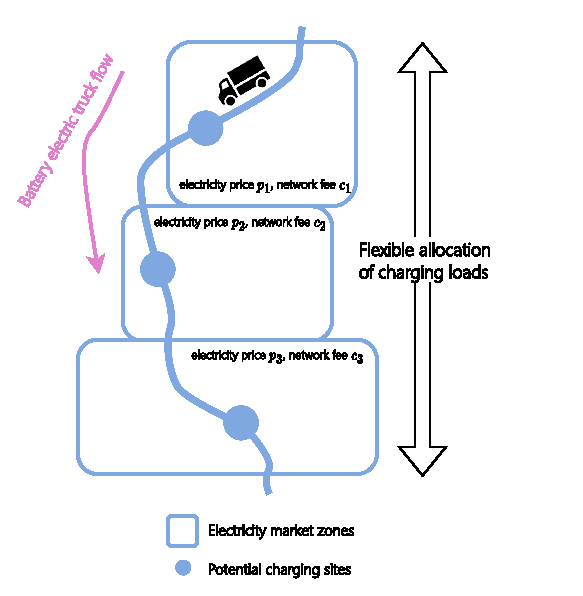
\includegraphics[width=0.6\linewidth]{images/interzonal_4.pdf}
              \caption{Illustration of flexible allocation of charging demand during long-haul trips of battery-electric trucks that pass through multiple regions of varying electricity prices and network fees, effecting costs of charging.}
              \label{fig:spatial_flex}
        \end{figure}

    \subsection{Model scope and assumptions}
        
        To address the research questions of this study, an optimization model is formulated that outlines the cost-optimal decarbonization of long-haul road freight trucking (see Figure \ref{fig:overview}). The model is a standard Network Design problem \citep{Yang01071998}. The model is formulated as a linear program to ensure the applicability of the model at large geographic scope. The decision making in this model reflects the perspective of a social planner.
        
        The core functionalities are summarized in the following: 
 
        \begin{itemize}
            \item \textbf{Representation of freight transport demand:} Following the classic Network Design Problem, the geography of the case study is conceptualized using a graph representation with nodes representing regions and edges transport connections. The transport demand is expressed based on origin-destination (OD)\footnote{Origin-destination data specifies the volume of tons transported between pairs of regions.} flows of freight goods. 
            
            \item \textbf{Technology and mode shift:} The transport demand is covered by vehicles of different modes, fuel types and drive-train technologies. These are characterized by different payload factors, energy efficiencies, and fueling needs. The mode and technology shifts follow substitution paths as defined by \citet{bakker2023stram}.
            
            \item \textbf{Vehicle stock modeling:} We include a detailed representation of the vehicle stock. This implies the modeling of the aging process of the fleet, along with the deteriorating efficiency, increasing maintenance costs, and, most importantly, the evolution of the technology developments of the battery, payload, and energy efficiency. It is important to note here that we associate each OD pair with a truck fleet that is exclusively traveling this route. This is in contrast to, for example, national freight transport model, such as the model by \citet{bakker2023stram}, where \enquote{fleet balancing} constraints ensure the efficient routing of vehicles within a closed system. In the present analysis, a corridor is modeled that connects multiple countries and intersects with other transport corridors. Therefore, the assumption of closed system boundaries is not applied here. 
             
            \item \textbf{Geographic allocation of charging load and infrastructure:}  The required charging infrastructure to cover the charging demand by the battery-electric is allocated and sized. The charging infrastructure is allocated under consideration of the limited driving range. Further, we consider multiple types of charging infrastructure. These differ by fueling speed and utilization factor. Overall, the allocation of the charging demands is determined by the following modeling features:
            \begin{itemize}
                \item \textbf{Mandatory breaks:} The maximum driving hours of truck drivers are considered. To do this the travel time along the route is endogenously mapped.
                \item \textbf{Battery state of charge:} The state of charge is modeled in spatial dimension, and, the amount of charged energy, as well as, the maximum driving time without charging is governed by the vehicle's battery's state of charge. 
                \item \textbf{Charging costs (volumetric):} Variable charging costs differ geographically based on the market-zone-dependent electricity costs.
                \item \textbf{Infrastructure costs (power):} Geographically varying annual network fees are considered in the capacity expansion. 
                \item \textbf{Adoption of battery electric trucks:} The adoption of BETs which is route-dependent.
            \end{itemize}

        \end{itemize}
        
        

        \begin{figure}[H]
              \centering
              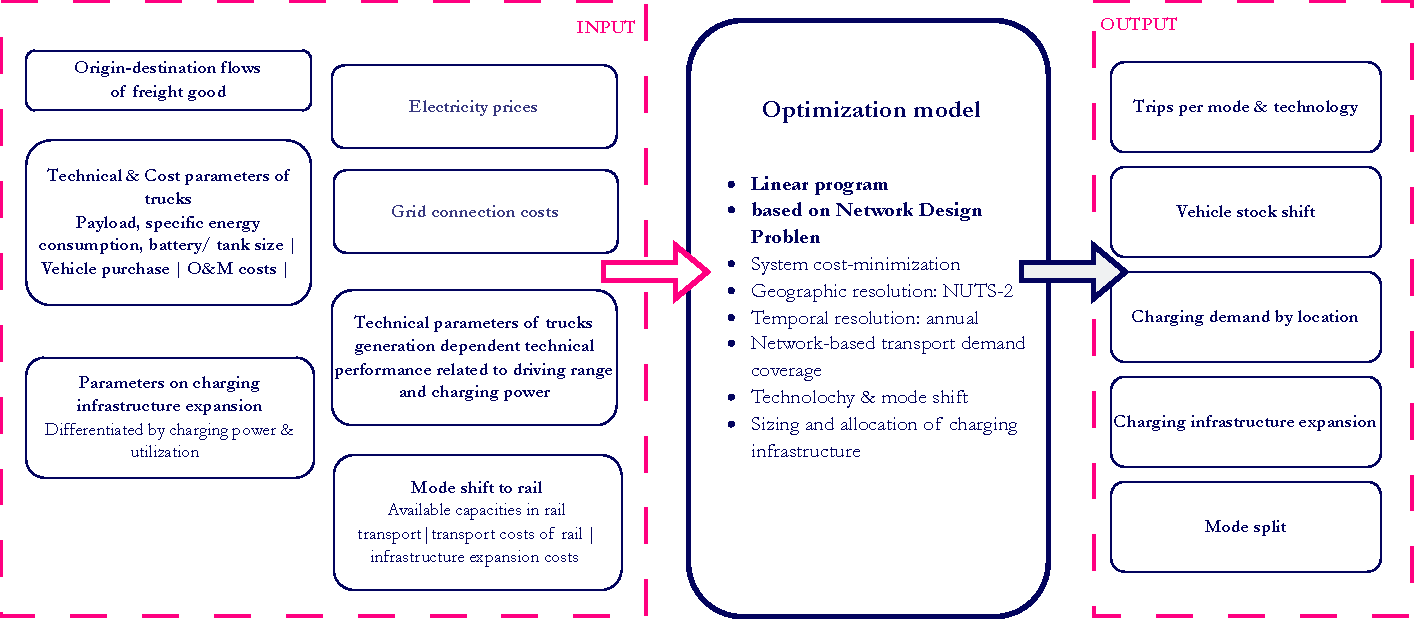
\includegraphics[width=1\linewidth]{images/flowchart_082025.drawio.pdf}
              \caption{Overview on the input and output parameters for the linear program. \hl{change this graphic}}
              \label{fig:overview}
        \end{figure}

        % The main output variables encompass the development of the electrification of road freight transport on an annual basis. Within this, the vehicle stock development is included along with the required expansion of different charging infrastructure types. Moreover, the shift towards rail freight transport is mapped. 
        %\hl{Reference here to the input-output relations (Figure)}
    \subsection{Mathematical formulation of the linear program}
    Used indices, parameters and decision variables are described in Table \ref{tab: variables_and_parameters}. The objective of the linear program is a cost-minimization encompassing cost related essentially to the purchase of vehicles, their operation and required infrastructure (Equation \ref{equ:obj_fun}).
    %\hl{here insert a clearer and detailed objective function definition, emphasizing cost structure}
    \begin{flalign} \label{equ:obj_fun}
            \begin{split}
                \underset{x}{\mathrm{minimize}} z = {C}^{\mathrm{vehicle\_stock, total}} + {C}^{\mathrm{fueling, total}}  +  {C}^{\mathrm{fueling\_infrastructure, total}}\\ +  {C}^{\mathrm{mode\_infrastructure, total}} + {C}^{\mathrm{travel\_time}}
            \end{split}
         \end{flalign}
    \paragraph*{Demand coverage}
    For each OD pair, freight transport demand is given exogenously via the annual amount of tons that is transported, $F$. These transport flows are covered by different drive-train technologies and modes.
    \begin{equation} \label{equ:demand_cov}
        \begin{split}
            \sum_{m \in \mathcal{M}} \sum_{t \in \mathcal{T}_m} \sum_{g \in \mathcal{G}} f_{yrmtg} = F_{yr} \quad :  \forall y \in \mathcal{Y},  r\in \mathcal{R} 
        \end{split}
    \end{equation}
    

    \paragraph*{Vehicle stock sizing}
    Based on these flows, the vehicle stock is sized by following:
    \begin{flalign} \label{equ:fleet_size_demand}
        \begin{split}
             h_{yrtg} \geq \sum_{k \in \mathcal{K}_r} \sum_{e \in \mathbf{E}_k}  \sum_{n \in \mathcal{N}_k} \frac{L_e}{W_{tg} L^{\textrm {a}}_{tg}} f_{yrk(m = \mathrm{road})tg} \\ : \forall y \in \mathcal{Y}, r \in \mathcal{R}, t \in \mathcal{T}_m, g \in \mathcal{G}
        \end{split}
    \end{flalign}
    $g$ indicates here the year in which the vehicle is produced. This value is particularly relevant in this equation as it determines the average payload ($W$) and the annual driving range ($L^{\textrm {a}}$).

    \paragraph*{Vehicle stock aging}
    The vehicle stock is tracked by year of purchase (generation $g$) and evolves through a stock-flow balance. The total vehicle stock $hyrtgh_{yrtg}$ consists of existing vehicles from the previous period, minus retirements, plus new purchases:

\begin{flalign} \label{equ:stock_balance}
h_{yrtg} = h^{\mathrm{exist}}{yrtg} - h^{-}{yrtg} + h^{+}_{yrtg} \quad : \forall y \in \mathcal{Y}, r \in \mathcal{R}, t \in \mathcal{T}, g \in \mathcal{G}, g \leq y
\end{flalign}
Vehicles of generation $g$ that have not yet been produced cannot exist:
\begin{flalign} \label{equ:no_future_gen}
h_{yrtg} = 0 \quad : \forall y \in \mathcal{Y}, r \in \mathcal{R}, t \in \mathcal{T}, g \in \mathcal{G}, g > y
\end{flalign}
Vehicles that have exceeded their lifetime $\Lambda_{tg}$ are fully retired:
\begin{flalign} \label{equ:lifetime_exceeded}
h_{yrtg} = 0 \quad : \forall y \in \mathcal{Y}, r \in \mathcal{R}, t \in \mathcal{T}, g \in \mathcal{G}, (y - g) > \Lambda_{tg}
\end{flalign}
For vehicles within their lifetime, the existing stock carries over from the previous period:
\begin{flalign} \label{equ:stock_carryover}
h^{\mathrm{exist}}{yrtg} = h{(y-\Delta)rtg} \quad : \forall y \in \mathcal{Y} \setminus {y^{\mathrm{init}}}, r \in \mathcal{R}, t \in \mathcal{T}, g \in \mathcal{G}, g < y, (y-g) \leq \Lambda_{tg}
\end{flalign}
New vehicles can only be purchased in their year of production:
\begin{flalign} \label{equ:new_purchases}
h^{+}_{yrtg} = 0 \quad : \forall y \in \mathcal{Y}, r \in \mathcal{R}, t \in \mathcal{T}, g \in \mathcal{G}, g \neq y
\end{flalign}
In the initial year, the existing stock for past generations is given exogenously:
\begin{flalign} \label{equ:initial_stock}
h^{\mathrm{exist}}{y^{\mathrm{init}}rtg} = H^{\mathrm{init}}{rtg} \quad : \forall r \in \mathcal{R}, t \in \mathcal{T}, g \in \mathcal{G}, g < y^{\mathrm{init}}
\end{flalign}
where $\Delta$ denotes the time step between modeled years, $y^{init}$ is the initial year, and $H^{init}_{rtg}$ is the exogenously given initial vehicle stock.

    % Further equations related to the aging and the changes in the vehicle stock are in the Appendix \hl{\dots}. 
    %\hl{make a small plots for mandatory break allocation, explanation what is shown}
    % \paragraph*{Spatial fueling flexibility}
    % In the allocation of fueling demand, the three following subsets are substantial for the definition of the equations:
    % \begin{itemize}
    %     \item $\mathbf{E}_k = (e_{k,1}, e_{k,2}, \dots, e_{k,a_k})$ defines the sequence of visited geographic locations along the path $k$. 
    %     \item Based on this, we define the following set of subsets: 
    %     \begin{equation}
    %         \mathcal{N}_{ktg}(R_{tg}) = \left\{\mathcal{N} \subseteq \mathbf{E}_k |\underset{x,y \in \mathcal{N}}{\max} d(x, y) \le R_{mtg}  \right\}
    %     \end{equation} 
    %     $N_{kmtg}$ contains all subsets of $\mathbf{E}_k$ that lie within the driving range of a vehicle ($R$). The driving range is dependent on the technology $technology$ and the generation of the vehicle $g$.
    %     \item Derived from the ordered sequence of the visited nodes, we define $\mathcal{U}_k=\left\{ e_{k,1}, e_{k,2}, \dots, e_{k,j}) | j = 1, 2, \dots, a_k \right\}$. $\mathcal{U}_k$ contains again subsets of $\mathbf{E}_k$ but is not dependent here on technical parameters of the drive-train. $\mathcal{U}_k$ contains all possible ordered sequences of $\mathbf{E}_k$ which contain the location of the destination of the path, $e_{k,1}$.
    % \end{itemize}
    % These are the building blocks for the three equations that define the allocation of fueling demand in the model.
    % Decision variable $s$ expresses the amount of fueled energy along the trip $r$ at the different geographic locations that are visited along the a path, $E_k$.

    % Equation \ref{equ_d:_fuel_2} defines that the sum of all fueled energy along the path needs to be equal to the demand that is define via the specific demand $D^{\mathrm{spec}}$ and the payload related to the drivetrain $W$. 

    % \begin{flalign} \label{equ_d:_fuel_2}
    %     \begin{split}
    %           \sum_{l \in \mathcal{L}_t} \sum_{e \in \mathbf{E}_{k} } s_{yrkmtlge} = \sum_{g \in \mathcal{G}} \frac{D^{\textrm{spec}}_{mtg} L_{k}}{W_{mtg}} f_{ykmtg} \\  : \forall y \in \mathcal{Y}, r\in \mathcal{R}, k \in \mathcal{K}_r,  m \in \mathcal{M}, t \in \mathcal{T}_m, g \in \mathcal{G}
    %     \end{split}
    % \end{flalign}
    % \hl{\textbf{initial SOC 100\% and end SOC 50\%; statt 0\%}; argument: damit man nie strandet}

    
    % It is important to note here, that the left siFfide of the equation does not include the summation over all visited locations along the route, $e \in \mathcal{E}_k$, as in \ref{equ_d:_fuel_2}. When path lengths are longer than the driving range associated with a technology, Equation \ref{equ_d:_fuel} is a tighter definition for the allocation of the demand as it ensures that within the subsets in $\mathcal{N}_{kmtg}$, the demand is covered. 
   \paragraph*{State of charge} Equations \ref{equ:_tank_cap} describe the state of charge along a route. In analogy to time-dependent battery state of charge equations, this set of equations describes the change in spatial dimension.
         \begin{flalign} \label{equ:_tank_cap}
        \begin{split}
            soc_{yrtge_{r, 1}} = SOC^{init} * Q^{batt}_{tg} \\
            soc_{yrtge_{r, i}} = soc_{yrtge_{r, i-1}} + s_{yrtlge_{r, i}} -  \sum_{g} D^{\mathrm{spec}}_{tg}L_{ke_{(i-1, i)}} * h_{yrtg} \\
            soc_{yrtge_{r, a}} \geq SOC^{final} * Q^{batt}_{tg}\\
            soc_{yrtge_{r, i}} \in \left(0;Q^{batt}_{tg}\right)
        \end{split}
    \end{flalign}

    The state of charge is increased by charged or fueled energy on-site and reduced by electricity consumption while driving between the past ($e_ {r,i-1}$) to the current geographic location ($e_ {r,i}$).

    \paragraph*{}
    
    \paragraph*{Travel time} Similar to the state of charge, the travel time of the fleet along a route is tracked by:
        \begin{flalign} \label{equ:_tank_cap}
        \begin{split}
            travel\_time_{yrtge_{r, 1}} = 0 \\
            travel\_time_{yrtge_{r, i}} = travel\_time_{yrtge_{r, i-1}} +\frac{s_{yrtge_{r, i}}}{\hat{P}_{tg}} +  \sum_{g} \frac{L_{ke_{(i-1, i)}}}{speed}  h_{yrmtg} + break\_time^+_{yrtge_{r, i}}\\
        \end{split}
    \end{flalign}
    Additional break time $break\_time^+$ is the difference between the total break time and the time to take for charging. 

    \paragraph*{Mandatory break taking} The mandatory breaks are imposed at geographic locations at which the break is required to happen at the latest. 
    \begin{flalign}
        \begin{split}
            travel\_time_{yrtge_{r, j}} \geq TravelTime^{min}_{e_{r, j}}
        \end{split}
    \end{flalign}
    
    
        \paragraph*{Sizing and allocation of fueling infrastructure}
    Index $l \in \mathcal{L}^{t}$ implies different fueling infrastructure for a technology. Parameter $\gamma_l$ translates the entire annual fueling demand to the required capacity to be installed. The installation of the charging infrastructure follows a defined subset of investment periods, $y \in \mathcal{Y}^{\textrm{exp}}$.  

   
    \begin{flalign}
\label{equ:cap_fuel_e_c}
\begin{split}
  Q^{\mathrm{charg\_infr}}_{ t e} + \sum_{y' \in \mathcal{Y}^{\mathrm{exp}}_y} q^{+, \mathrm{charg\_infr}}_{y'te}
  \;\ge\; \gamma_l^{\mathrm{charg\_infr}}
  \sum_{r \in \mathcal{R}} \sum_{k \in \mathcal{K}_{re}} \sum_{g \in \mathcal{G}}  s_{y r t e g} \\\qquad\forall\, y\in\mathcal{Y},\;  t\in\mathcal{T},\; m\in\mathcal{M},\;  e\in\mathcal{E}
\end{split}
\end{flalign}

    
    \paragraph*{Expansion of mode infrastructure}
    Similar to this, the mode infrastructure is established:
    \begin{flalign} \label{equ:mode_infrastr_e}
        \begin{split}
             Q^{\mathrm{mode\_infr}}_{me}  +  \sum_{y' \in \mathcal{Y}^{\mathrm{exp}}_y} q^{+, \mathrm{mode\_infr}}_{y'me} \geq  \gamma^{\textrm{mode\_infr}}_m \sum_{r \in \mathcal{R}} \sum_{k \in \mathcal{K}_{re}} \sum_{t \in T_{m}}\sum_{g \in \mathcal{G}}  f_{yrkmtg} \\: \forall y \in \mathcal{Y}, m \in \mathcal{M}, e \in \mathcal{E}
        \end{split}
    \end{flalign}
    \\

    
    \subsection{Code availability}
    This model is implemented using Julia \citep{bezanson2017julia} und JuMP package \citep{Lubin2023} for the formulation of the model. Gurobi Optimizer version 12.0.3 is used for solving the linear program \citep{gurobi}. The code is open-source available on \url{https://github.com/antoniamgolab/iDesignRES_transcompmodel.git}.
     
   %  \hl{how is travel time treated},\cite{csender2021}: 4.5 hours are not the rule; empirical evidence is here
    

    % Please add the following required packages to your document preamble:
% \usepackage{booktabs}
% \usepackage{graphicx}
\begin{table}[]
\centering
\caption{Sets, decision variables and parameters used for the formulation of the linear program. }
\label{tab: variables_and_parameters}
\resizebox{\textwidth}{!}{%
\begin{tabular}{@{}lll@{}}
\toprule
Notation                    & Description                                                                                                              & Unit   \\ \midrule
$y \in \mathcal{Y}$         & year                                                                                                                     &        \\
$r \in \mathcal{R}$     & origin-destination pair & \\ 

$m \in \mathcal{M}$ & transport modes & \\
$t \in \mathcal{T}_m$         & drive-train technology                                                                                              &        \\
% $l \in \mathcal{L}_t$       & type of fueling infrastructure                                                                                  &        \\
$e \in \mathcal{E}$         & geographic location                                                                                                                     &        \\
$\mathcal{Y}^{\mathrm{exp}}$             & set of years of investment decision for infrastructure expansion                                                                                                        &        \\
$\mathcal{Y}_y$             & set of years until year $y$                                                                                               &        \\
$\mathbf{E}_k = (e_{k,1},e_{k,2}, \dots, e_{k,a} )$         & sequence of visited geographic locations along path $k$                                                                                                                &        \\
 \midrule
$f_{yrkmtg}$                   & \begin{tabular}[c]{@{}l@{}}transport volumes\end{tabular}  & T/a     \\
$h_{yrmtg}$                   & number of vehicles  in the vehicle fleet&      \\
$h^{\mathrm{+}}_{yrmtg}$                   & number of vehicles added to the fleet  &      \\
$h^{\mathrm{-}}_{yrmtg}$                   & number of vehicles exiting the fleet  &      \\



$s^{fueling}_{ykte}$ &
  \begin{tabular}[c]{@{}l@{}} annual fueling demand \end{tabular} &
  MWh/a \\
  $soc_{ytge}$ & state of charge of truck fleet    & kWh     \\
  $travel\_time_{ytge}$ & accumulated travel time of fleet   & kWh     \\
  $break\_time^+_{ytge}$ & time spent on break without fueling/charging   & kWh     \\
  
$q^{+, \mathrm{fuel\_infr}}_{yte}$   & added fueling infrastructure capacity & MW     \\
$q^{+, \mathrm{mode\_infr}}_{yme}$ & added fueling infrastructure capacity    & MW     \\ 

\midrule
$F_{yr}$                    & freight transport demand                                                               & T      \\
$D^{\mathrm{spec}}_{tg}$             & \begin{tabular}[c]{@{}l@{}}specific energy consumption\end{tabular}          & MWh/km \\
$W_{tg}$                    & average payload load                                                                & T      \\
$Q^{\mathrm{batt}}_{tg}$                    & battery/tank capacity                                                            & MWh     \\

$SOC^{init}$                    & initial state of charge of battery/tank level 
& \%     \\
$SOC^{final}$                    & final state of charge of battery/tank level 
& \%     \\
$R_{mtg}$                    & maximum driving range                                                          & km     \\

$L^{\mathrm{a}}_{mtg}$                       & annual driving range                                                                                                      & km     \\
$L_e$                       & driving distance at a geographic location                                                                                                      & km     \\
$L_e$                       & driving distance at a geographic location                                                                                                      & km     \\
$Q^{\mathrm{charg\_infr}}_{te}$       & initial fueling capacity                                                            & kW     \\
$Q^{\mathrm{mode\_infr}}_{me}$     & inital transport capacity                                                                      & kW     \\

$\gamma^{\mathrm{charg\_infr}}_l$                    & \begin{tabular}[c]{@{}l@{}}ratio between of demand of annual peak hour of charging infrastructure \\ utilization and total annual demand\end{tabular}                                                                           &  MW/MW     \\
$\gamma^{\mathrm{mode\_infr}}_l$                    & \begin{tabular}[c]{@{}l@{}}ratio between of demand of annual peak hour of mode infrastructure \\utilization and total annual demand\end{tabular}                                                                          &  Tkm/Tkm      \\
\bottomrule
\end{tabular}%
}
\end{table}
%     \newpage 
%     \subsection{Data preparation: Road freight decarbonization in the the Scandinavian-Mediterranean corridor}

        
            
        
%         \subsubsection{Drive-train technologies}

%         As we focus on the electrification of the truck fleet, we limit the technology portfolio for truck drive-trains to two technologies: diesel-fueled combustion engine and battery-electric. Per technology, we consider one representative vehicle type each. For the rail mode, we exclusively consider electric drive-trains. 

%         Relevant costs for the truck drive-train technologies are comprised in Table \hl{\dots}. Costs for the purchase of the vehicle and maintenance \& repair (M\&R) vary by technology and are levelized by a vehicle's mileage to a tonne per km. For each route, the total driver costs are evaluated depending on the route's length, the average driving speed, and, further, also considering required fueling time. For the latter, we also consider whether this re-fueling takes longer than the compulsory break of 45min each 4.5 of trip time \citep{WKO_Arbeitszeit}. 
%         \hl{include the case of multiple drivers}
%         \hl{how much of the battery is tanked/charged? in which constraints is this reflected?}
%         \subsubsection{Electricity prices and grid connection costs}

%         The fuel costs for BEVs are directly drawn from the electricity prices which vary depending on the electricity market zone. We simplify the electricity market zones by directly relating these to the countries, assuming one unique electricity price per country. We thereby neglect the the multiple electricity market zones in Sweden, Norway in Italy. The relevant electricity prices are drawn from shadow prices of the demand coverage constraint from the electricity market model EMPIRE \citep{OpenEMPIRE, BACKE2022100877}. The country-dependent network fees are drawn from the work of \citet{Lanz2022} and are assumed to stay constant over the entire time horizon. Table \hl{\dots} displays an overview on these values. 
%             \hl{MANDATORY BREAK CAN BE SPLIT!}
%         \subsubsection{Charging infrastructure} \mbox{}\\
            
%             % Please add the following required packages to your document preamble:
% % \usepackage{booktabs}
% % Please add the following required packages to your document preamble:
% % \usepackage{booktabs}

%             Table \ref{tab:cs_types} refers to utilization factor and cost parameters

%             Costs for charging infrastructure are assumed to drop throughout the years \citep{transportandedecarb2021}. 

%             \hl{How to differentiate in the model between charging types endogeneously?}
            
%             \hl{todo: include a table for overview on charging infrastructure: kW; max. utilization rate; }

%                 \subsubsection{Shift from road to rail freight}
%         The rail mode is simplified in the present analysis by reducing the representation of the costs to the following two components: 
%         \begin{itemize}
%             \item \textbf{Levelized transport costs:} These costs refer to the linehaul costs and comprise levelized costs for the rail operation, fuel, train and wagon, and labor costs. 
%             \item \textbf{Terminal costs:} These are costs for the on and off-loading of freight goods on a train. 
%             \item \textbf{Rail infrastructure expansion costs:} These costs refer to the expansion of rail infrastructure that is needed to transport an additional unit of freight per km. 
%         \end{itemize}
    
%         Table \hl{\dots} summarizes the parametrization for costs of rail freight.
%     \textit{No explicit intermodality modeled here as the rail infrastructure is parallel to road infrastructure for the most part and rail becomes more costcompetitive with distance}

%    \subsection{Case studies}
%     \hl{include }
%     To quantify the magnitude of charging infrastructure capacity that is affected by the geographically varying installation and electricity costs, four case studies are designed. An overview of these is given in Table \ref{tab:ass_install_elecprices}. The symbol $\sim$ is used to express that a parameter is kept constant over all considered geographic regions. The symbol $\uparrow \downarrow$ indicates that the geographic variation of the parameter is considered. A base case, \textit{Case 1}, is defined where the values for these parameters are kept constant over all regions. \textit{Cases 2} and \textit{3} are for isolating the impacts of these two parameters separately, while in \textit{Case 4} finally includes a geographic variation of both.
%     % Please add the following required packages to your document preamble:
% % \usepackage{booktabs}
%         \begin{table}[H]
%         \centering
%         \caption{Overview of the assumptions by case study for the parametrization of installation costs for charging infrastructure and electricity prices by country: The symbol $\sim$ indicates constant values for all regions. The symbol $\uparrow\downarrow$ indicates the consideration of variations of these parameters.}
%         \label{tab:ass_install_elecprices}
%         \begin{tabular}{@{}lll@{}}
%         \toprule
%         \textbf{Case studies} & \textbf{Network fees (\euro/MWpeak)} & \textbf{Electricity prices(\euro/MWh)} \\ \midrule
%         \textit{Case 1}       & $\sim$                      & $\sim$                      \\
%         \textit{Case 2}       & $\uparrow \downarrow$       & $\sim$                      \\
%         \textit{Case 3}       & $\sim$                      & $\uparrow \downarrow$       \\
%         \textit{Case 4}       & $\uparrow \downarrow$       & $\uparrow \downarrow$       \\ \bottomrule
%         \end{tabular}
%         \end{table}
%             \newpage 
            
%         \subsubsection{Cost parameters}
%             Tables \ref{tab:ass_fuel_costs}, \ref{tab:ass_fleet_parameters} and \ref{tab:fueling} summarize all parameters assumed for the estimation of the cost parameters used in this analysis. 

%             \paragraph*{Fuel costs} \mbox{}\\ 
%                 Diesel is assumed to have a constant price throughout all considered regions. Additionally to the diesel price, a carbon price is added. This is drawn from the OpenEntrance project \citep{auer2020quantitative}. The electricity price is varied at the country level. For this, shadow prices of demand coverage constraint calculated with the EMPIRE electricity market model are used \citep{BACKE2022100877, OpenEMPIRE}. 
                
%             \paragraph*{Fleet-related costs} \mbox{}\\
                            




                
                
%                 % Figure \dots illustrate the considered supply options for the delivery of fuel to the charging or fueling station. The supply of diesel and fueling infrastructure is assumed to be established to cover the full existing demand for diesel along the corridor. Delivery costs are directly included in the diesel price. 

%                 % In the build-up of charging infrastructure for battery-electric trucks, significant reinforcements of the power grid connection are needed. These are represented with a value for network provision charge [REF]. 

%                 % These are assumed to be constant throughout the total case study area. However, grid reinforcement needs have been described to vary locally significantly [REF]. These potential local differences are here neglected though due to the following two reasons: (1) no data at distribution grid level, (2) geographic resolution.

%                 % For the delivery of hydrogen to a refuelling station, is assumed to have different options for which costs also vary in time: Pipeline delivery, on-site production using a grid-connected electrolyser and truck delivery [REF Lundblad, Nugruhu]. The pipeline delivery is assumed to be available as of 2030, until which a central hydrogen pipeline network is planned to be established, the European Hydrogen Backbone. Based on the development plans, the relative distances between the edges of the road network and the EHB pipeline are evaluated and dictate the required investment costs to establish a pipeline connection between the refueling station and the EHB. Costs for the on-site production include the network provision charge and an electrolyzer. Finally, costs for the truck delivery are directly added to the variable transport cost component.  

%                 % https://energy.ec.europa.eu/topics/markets-and-consumers/market-legislation/hydrogen-and-decarbonised-gas-market-package_en
%                 % \begin{itemize}
%                 %     \item what energy prices are considered?
%                 %     \item what is the source of them?
%                 %     \item what is the local variation in them? and why?
%                 %     \item why is hydrogen varied? 
%                 %     \item how is it varied (the scenarios)?
%                 % \end{itemize}
 

%     % \subsection{Limitations}
%     %     \begin{itemize}
%     %         \item limitations due to setting the system boundary
%     %         \item limitations due to not considering seasonality in energy prices and transport volumes 
%     %         \item no roundtrips assumed just one route driven by same fleet
%     %         \item driving range changes in time, no tracking of WHEN a different drivetrain has been implemented, range just increases 
%     For the sizing of charging infrastructure, we quantify $\alpha_{yl}$ using the following formula: 
%     \begin{flalign} \label{equ:infr_sizing}
%         \begin{split}
%              \gamma_{yl} = \textsc{share of traffic during day peak} \times \hat{Cap}_{yl}\frac{1}{365}
%         \end{split}
%     \end{flalign}
%     \subsection{Day versus night overnight charging}
%     \hl{\textbf{as inspired by} } \citep{SHOMAN2023103825}
% \hl{IT und NO als limitations sind nur als eine Marktzone; Es geht um die unterschiedlichen Preiszonen}
% \hl{national vs. internationaler verkehr}
% \hl{Future work wäre f.e. zonensplit effekt auf die verschiebung der Strommengen/Ladeinfrastruktur}
% \hl{Day and night charging type - two technologies --- but then decided based on what? }
% \hl{include clear statement why not catenary}
    
\newpage

\section{Case study: Scandinavian-Mediterranean corridor}
    \subsection{The Scandinavian-Mediterranean corridor}
        The Scandinavian-Mediterranean corridor represents a North-South axis within the Trans-European Transport Network (TEN-T) \citep{EU_TEN_T}. It includes parts of the European road and rail network that connect Norway and Finland through Sweden, Denmark, Germany, Austria, and Italy, extending to Sicily. Part of the corridor is also allocated in the South of Finland, which is connected through maritime waterways and airports to the major part of the corridor\footnote{Given the wide extent of this corridor, no image outlining its allocation and its course is included in this manuscript. Please refer to \citep{EU_TEN_T_Maps} for an overview.}. Overall, the corridor connects 19 international airports and 25 seaports positioned along the European coastline. The core network encompasses over 6,300 km of road and 9,400 km of rail transport infrastructure \citep{EU_SCM_Corridor_Study}. 

        The extent of this corridor is used in this work for the definition of the area of the case study. While the road network of the Scandinavian-Mediterranean corridor connects major demand centers in the given countries, in the present analysis, we also include road transport infrastructure that is not directly part of the corridor infrastructure as the official classification: We also include road infrastructure aside from this that is allocated within the connected regions. Therefore, the extent of the case study was set to all NUTS-2 regions \footnote{using the following NUTS definition: \citep{EU_Eurostat_NUTS}} intersected by the Scandinavian-Mediterranean road infrastructure. In total, 4621 nodes are included in the analysis.
    \subsection{Transport activity}
        
        To estimate the transport activity along the road network of the Scandinavian-Mediterranean corridor, the data prepared within the context of the ETISplus project was used \citep{Speth2021}. This data includes projections for transport flows for road freight for the year 2030. The relevant information in this data set used for the present work includes the following: (1) Origin-Destination nodes with the geographic granularity of NUTS-3 level, (2) yearly aggregated tons transported between these nodes, (3) the route course with a geographic resolution of NUTS-3 level. This data is aggregated to NUTS-2 level, and filtered for exclusively international routes. A small number of transport routes was reduced by filtering the routes by $\geq 100$ tons and a minimum route length of 360 $km$, similar to the study of \citet{SHOMAN2023103825}. This results in 81 considered NUTS-3 regions and 2,043 OD pairs. The optimization horizon is 2020-2060, while the focus of the analysis in this work is 2020-2050. This is done to avoid artifacts in the technology choices that occur at the end of the optimization horizon, where investment decisions are made without foresight for future operational years. Based on the reference year the data was determined for, 2030, the transport demand is extrapolated based on historic growth of freight road transport activity \citep{eurostat2024roadfreight} The transport performance grows between 2020 to 2060 from 7.63 Btkm to 8.93 Btkm. Mandatory breaks are determined for each of the OD pairs similar to how this is determined in the paper of \citet{SHOMAN2023103825}.

        
    \subsection{Cost parameters}
    
    \subsubsection{Drive-train technologies}
        Table \ref{tab:ass_fleet_parameters} describes cost assumptions and its sources for internal combustion engine trucks and BETs. 
                % Please add the following required packages to your document preamble:
% \usepackage{booktabs}
    \begin{table}[H]
    \centering
    \caption{Network fees assumed constant over time \citep{Lanz2022}.}
    \label{tab:elec_networkfees}
    \begin{tabular}{@{}lr@{}}
    \toprule
    \textit{Country} & \textbf{Network fees (\euro/kW/a)} \\ \midrule
    \textit{Austria}  & 14.69 \\
    \textit{Denmark}  & 12.80 \\
    \textit{Finland}  & 12.33 \\
    \textit{Germany}  & 16.77 \\
    \textit{Italy}    & 8.96  \\
    \textit{Norway}   & 8.58  \\
    \textit{Sweden}   & 12.19 \\ \bottomrule
    \end{tabular}
\end{table}
                % \begin{itemize}
                %     \item What supply infrastructures are considered? (figure!)
                %     \item what references are used? - including the EHB
                %     \item What are the costs? 
                %     \item Based on what are these retrieved/estimated?
                % \end{itemize}

            \begin{table}[H]
            \centering
            \caption{Assumptions on fleet-related parameters.}
            \label{tab:ass_fleet_parameters}
            \resizebox{\textwidth}{!}{%
            \begin{tabular}{llllrl}
            \hline
            Fleet-related costs and parameters & 2020                        & 2035                        & 2050                        & Unit                     & Reference \\ \hline
            \multicolumn{6}{l}{\textbf{Diesel-fueled combustion engine}}                                                                                                        \\
            Vehicle purchase                   & \multicolumn{1}{r}{105,484} & \multicolumn{1}{r}{115,252} & \multicolumn{1}{r}{115,252} & \euro                    &   \citep{transportandedecarb2021}        \\
            Maintenance \& Repair (M\&R) & \multicolumn{1}{r}{20,471} & \multicolumn{1}{r}{20,608} & \multicolumn{1}{r}{20,608} & \euro/a                       &      \citep{transportandedecarb2021}           \\
            Specific energy consumption  & \multicolumn{1}{r}{2.90}   & \multicolumn{1}{r}{2.65}   & \multicolumn{1}{r}{2.40}   & kWh/km                        &     \citep{MARTIN2023100156}            \\
            Emission factor              & \multicolumn{1}{r}{86}     & \multicolumn{1}{r}{79}     & \multicolumn{1}{r}{71}     & gCO\textsubscript{2}/Tkm      & \citep{UmeltbundesamtPDF} \\
            Tank size                          & \multicolumn{1}{r}{5600}    & \multicolumn{1}{r}{5600}    & \multicolumn{1}{r}{5600}    & kWh                      &  \citep{Speth2021}         \\
            Yearly mileage                     & \multicolumn{1}{r}{136,750} & \multicolumn{1}{r}{136,750} & \multicolumn{1}{r}{136,750} & km                       &       \citep{MARTIN2023113637}   \\
            Average load per truck                    & \multicolumn{1}{r}{13,6}                     & \multicolumn{1}{r}{13,6}                     & \multicolumn{1}{r}{13,6}                     & T                       &        \citep{SHOMAN2023103825}   \\
             \multicolumn{6}{l}{\textbf{Battery-electric}}  \\
            Vehicle Purchase                   & \multicolumn{1}{r}{220,000}                     &\multicolumn{1}{r}{177,381}                     & \multicolumn{1}{r}{146,293}                    & \euro                    &   \citep{basma2023tco}        \\
            Maintenance \& Repair (M\&R)       & \multicolumn{1}{r}{14,000}                      & \multicolumn{1}{r}{14,000}                      & \multicolumn{1}{r}{14,000}                      & \euro/a                  &       \citep{transportandedecarb2021}    \\
            Specific energy consumption        & \multicolumn{1}{r}{1.44}                        & \multicolumn{1}{r}{1.15}                        & \multicolumn{1}{r}{1.05}                        & kWh/km                   &   \citep{transportandedecarb2021}       \\
            Tank size                          & \multicolumn{1}{r}{560}                         & \multicolumn{1}{r}{1120}                        & \multicolumn{1}{r}{1400}                        & kWh                      &       \citep{transportandedecarb2021}    \\
            Yearly mileage                     & \multicolumn{1}{r}{136,750}                     & \multicolumn{1}{r}{136,750}                     & \multicolumn{1}{r}{136,750}                     & km                       &        \citep{transportandedecarb2021}   \\
            Average load per truck                    & \multicolumn{1}{r}{11,56}                     & \multicolumn{1}{r}{12,38}                     & \multicolumn{1}{r}{13,6}                     & T                       &        \citep{SHOMAN2023103825}   \\
            \hline
            \end{tabular}
            }
            \end{table}

            
           
    \subsubsection{Rail infrastructure}
    The rail mode is simplified in the present analysis by reducing the representation of the costs to the following components: 
        \begin{itemize}
            \item \textbf{Levelized transport costs:} These costs refer to the linehaul costs and comprise levelized costs for the rail operation, fuel, train and wagon, and labor costs. 
            \item \textbf{Terminal costs:} These are costs for the on and off-loading of freight goods on a train. 
            \item \textbf{Rail infrastructure expansion costs:} These costs refer to the expansion of rail infrastructure that is needed to transport an additional unit of freight per km. 
        \end{itemize}
        %\hl{insert table hre }
    \subsubsection{Charging infrastructure}
            Regard refueling infrastructure, we exclusively consider charging infrastructure, assuming that the refueling infrastructure for ICEV is of sufficient capacities and does not need to be expanded. 

            We model one representative charging infrastructure type with cost parameters presented in Table \ref{tab:fueling}.
            
            % The following two types of charging infrastructure are considered:
            % \begin{itemize}
            %     \item \textbf{Megawattcharging (MCS):} These type of chargers provide peak power levels of 1MW. These type of chargers provide fuel recharging during the 45min brakes. \citep{en16124704}
            %     \item \textbf{Slow overnight charging:} These are charging systems providing peak power levels of 100kW. The recharging is used during longer brakes of truck drivers.  
            % \end{itemize}
            \hl{https://pubsonline.informs.org/doi/10.1287/trsc.2016.0678} \\
            %\hl{\href{https://www.sciencedirect.com/science/article/pii/S2667259625000104#fig0003}}
    \begin{table}[H]
            \centering
            \caption{Assumptions of parameters related to the deployment of fueling infrastructure.}
            \label{tab:fueling}
            \resizebox{\textwidth}{!}{%
            \begin{tabular}{@{}llllll@{}}
            \toprule
            Charging-infrastructure-related parameters & 2020 & 2035 & 2050 & Unit          & Reference        \\ \midrule
            Charging station                          & 400  & 300  & 250  & \euro/kW      &        \citep{transportandedecarb2021} \\ \bottomrule
            \end{tabular}
            }
            \end{table}

    \subsection{Scenario definition}
        To account for uncertainties surrounding the future charging loads and their spatial allocation, we employ a factorial experimental design combining multiple uncertain parameters. The uncertainty analysis framework applies parameter variations to the base case preprocessing, generating 24 distinct scenarios (4 electricity price scenarios $\times$ 2 charging markups $\times$ 3 technology cost trajectories). Table~\ref{tab:uncertainty_parameters} summarizes the uncertain parameters and their levels.

        \begin{table}[H]
        \centering
        \caption{Summary of uncertainty parameters and factorial design. The full factorial yields $4 \times 2 \times 3 = 24$ scenarios.}
        \label{tab:uncertainty_parameters}
        \begin{tabular}{@{}llll@{}}
        \toprule
        \textbf{Parameter} & \textbf{Levels} & \textbf{Values} & \textbf{Source} \\ \midrule
        Electricity price scenario & 4 & Go RES, NECP, REPowerEU++, Trinity & \citep{loffler2025euenvis} \\
        Carbon price trajectory & 4 & Coupled with electricity scenario & \citep{loffler2025euenvis} \\
        Charging markup & 2 & 15\%, 30\% & \citep{Lanz2022} \\
        BET purchase cost trajectory & 3 & $-$30\%, 0\%, $+$30\% by 2050 & \\ \bottomrule
        \end{tabular}
        \end{table}
        \begin{table}[]
\centering
\caption{Technical assumptions of charging infrastructure.}
\label{tab:cs_types}
\begin{tabular}{@{}lrr@{}}
\toprule
Charging infrastructure type     & Output & Max. utilization rate \\ \midrule
\textbf{Megawatt charging (MCS)} & 1MW    & 30\%                  \\
\textbf{Slow charging}           & 100kW  & 30\%                  \\ \bottomrule
\end{tabular}
\end{table}

        \subsubsection{GENeSYS-MOD electricity price scenarios}
        To capture uncertainty in future electricity prices, we use four scenarios from the GENeSYS-MOD EU-EnVis-2060 framework \citep{EUEnVis2025}: \textit{Go RES} (ambitious renewable expansion achieving carbon neutrality before 2050), \textit{NECPEssentials} (extension of current national energy and climate plans), \textit{REPowerEU++} (self-sufficient European energy system), and \textit{Trinity} (internal EU divisions affecting climate ambition). Each scenario embeds an internally consistent carbon budget constraint that determines both the electricity generation mix and resulting wholesale prices. Country-specific and year-specific electricity price ratios are applied relative to the Go RES baseline, preserving the temporal trajectory of each scenario. Compared to Go RES, the alternative scenarios yield average electricity prices of approximately 70\% (NECPEssentials), 66\% (REPowerEU++), and 62\% (Trinity).
        % \hl{Show an image displaying the relative levels by scenario}
        \subsubsection{Carbon price trajectories}
        Each GENeSYS scenario is associated with a distinct carbon price trajectory reflecting its climate ambition level (Table~\ref{tab:carbon_trajectories}). Carbon prices are interpolated annually to provide consistent year-by-year values synchronized with each electricity price scenario, maintaining internal consistency between energy system decarbonization and carbon pricing.

        \begin{table}[H]
            \centering
            \caption{Carbon price trajectories by GENeSYS-MOD scenario (\euro/tCO\textsubscript{2}).}
            \label{tab:carbon_trajectories}
            \begin{tabular}{@{}lrrrr@{}}
            \toprule
            \textbf{Scenario} & \textbf{2020} & \textbf{2030} & \textbf{2040} & \textbf{2050} \\ \midrule
            Go RES & 30 & 200 & 500 & 1000 \\
            REPowerEU++  & 30 & 150 & 350 & 700 \\
            NECPEssentials  & 30 & 100 & 250 & 500 \\
            Trinity  & 30 & 80 & 180 & 350 \\ \bottomrule
            \end{tabular}
        \end{table}

        \subsubsection{Charging and fuel cost parameters}
        \paragraph*{Charging infrastructure markup.} The charging infrastructure markup represents the margin charged by Charging Point Operators (CPOs) on top of wholesale electricity costs, covering equipment amortization, maintenance, grid connection fees, and profit margin. Based on the levelized cost of charging framework by \citet{Lanz2022}, two markup levels are tested: 15\% representing a competitive mature market with depot charging and high-volume contracts, and 30\% representing current public charging conditions consistent with observed pricing at major European truck charging networks.

        \subsubsection{Technology cost uncertainty}
        To account for uncertainty in future BEV costs (battery packs, electric drivetrains), a time-dependent uncertainty approach is applied. Near-term BEV costs (2020--2030) are well-constrained by current market data and announced production plans, while long-term costs (2040--2060) are subject to greater uncertainty regarding technological breakthroughs and learning curves. Therefore, the technology cost multiplier grows linearly from no deviation in 2020 to $\pm$30\% by 2060, yielding three trajectories: optimistic ($-$30\% by 2060), reference (no deviation), and pessimistic ($+$30\% by 2060).

        \subsubsection{Spatial relocation mechanisms}
        Two mechanisms are evaluated for their effectiveness in redistributing charging loads along the corridor (Table~\ref{tab:relocation_mechanisms}). These levers operate through different cost channels and affect both the spatial distribution of charging infrastructure and the aggregate level of electrification. These are particularly applied at the 

        \begin{table}[H]
        \centering
        \caption{Spatial relocation mechanisms and their effects on charging load distribution.}
        \label{tab:relocation_mechanisms}
        \begin{tabular}{@{}p{2.8cm}p{3.5cm}p{3cm}p{4cm}@{}}
        \toprule
        \textbf{Mechanism} & \textbf{Cost channel} & \textbf{Primary effect} & \textbf{Expected outcome} \\ \midrule
        Electricity price differentiation & Variable costs (per-kWh) & Spatial arbitrage & Incentivizes charging in lower-price regions; effect scales with charging volume \\
        \addlinespace
        Network fee differentiation & Fixed costs (per-kW) & Infrastructure siting & Affects economic attractiveness of charging infrastructure deployment; stronger effect on high-capacity stations \\
        \bottomrule
        \end{tabular}
        \end{table}

        \subsection{Border region}
        %Modal shift to rail is route-dependent, with competitiveness determined by the trade-off between terminal costs (fixed per shipment) and linehaul costs (proportional to distance). Rail becomes increasingly competitive with distance as the fixed terminal costs are amortized over longer hauls.

\section{Results}
    \hl{Preliminary results} \\
    
    \subsection{Technology adoption}
    Figures \ref{fig:average_adoption_by_scenario} and \ref{fig:odpair_diffs} display how the battery electric truck fleet changes by the different settings of electricity price scenarios. The 24 intitial scenarios are here grouped by electricity price scenarion and the average of the fleet sizes are displayed. Figure \ref{fig:average_adoption_by_scenario} displays the absolute numbers of BET adoption along the entire corridor. The absolute values do not vary significantly. Figure \ref{fig:odpair_diffs} shows differences by OD pair matrix. The routes are here categorized by origin and destination countries. We see here differences in the adoption, particularly in the bottom row which compare the three of the scenario to the \textit{Reference} scenario GO RES. GO RES reflect high share of renewable energy sources adoption. The differences are here particularly seen in the OD pair connections Norway-Sweden, Italy-Germany and Italy-Germany, and Austria-Italy/Italy-Austria.
    \begin{figure}[H]
          \centering
          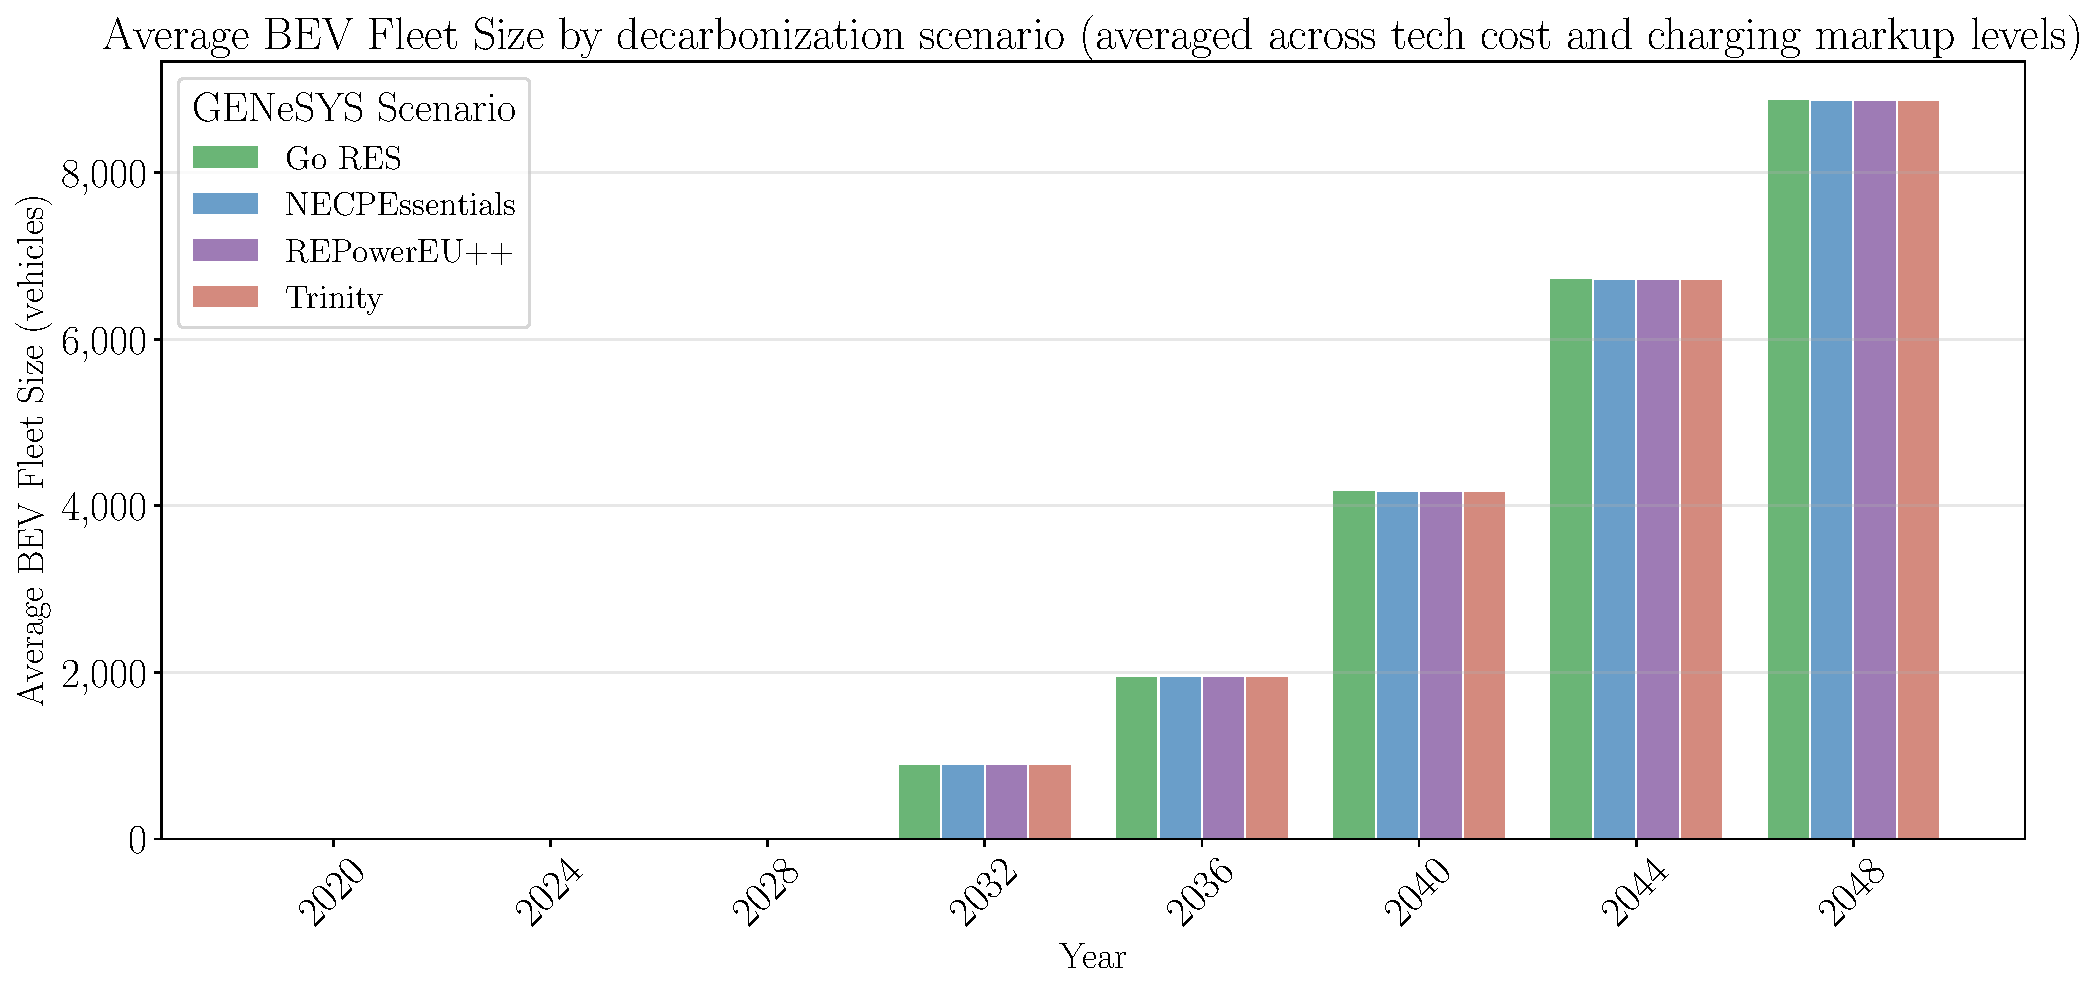
\includegraphics[width=0.8\linewidth]{images/absolute_bev_fleet_by_genesys.pdf}
          \caption{BET fleet size by decarbonization scenario}
          \label{fig:average_adoption_by_scenario}
    \end{figure}
    \begin{figure}[H]
        \centering
        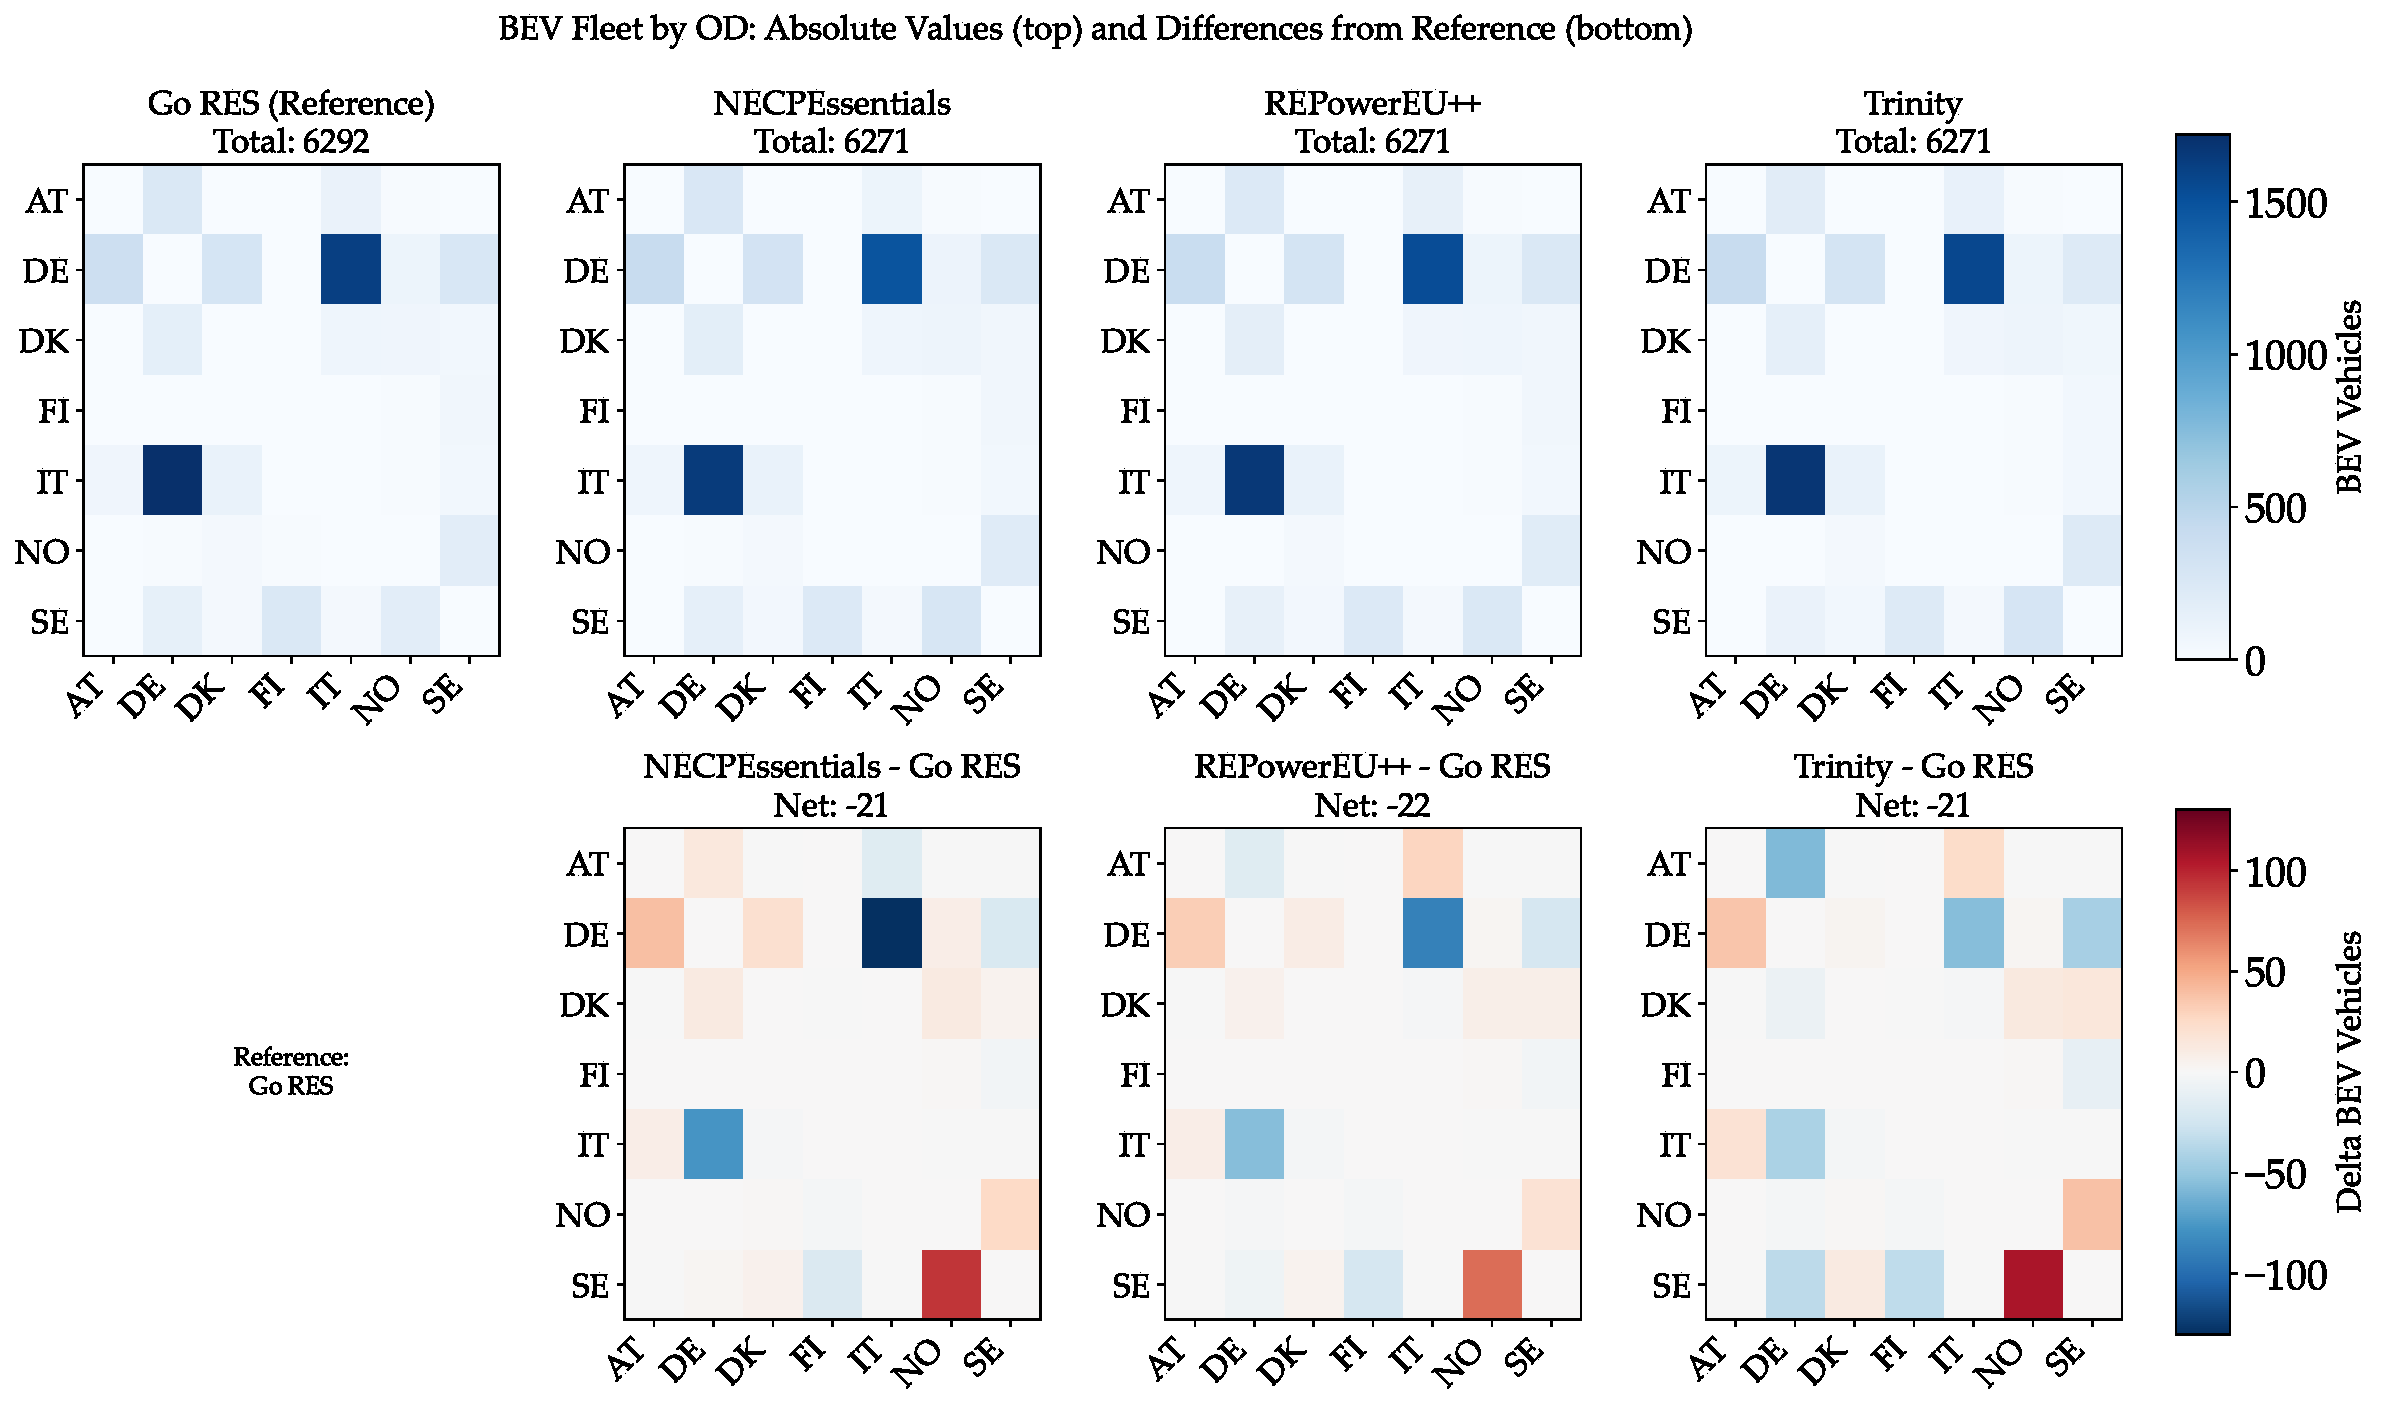
\includegraphics[width=\linewidth]{images/bev_od_matrices_with_deltas_2040.pdf}
        \caption{Differences in the BET adoption by origin-destination countries by 2048. The bottom row displays the differences to the GO RES scenario.}
        \label{fig:odpair_diffs}
    \end{figure}
    % Results showing the turnover towards BEVs in the truck fleet across different scenarios
    % What factors impact the pace and extent of BEV adoption?

    
       % \begin{itemize}
    %     \item Figure 1: BET fleet growth --- span over all scenarios 
    %     \item Figure 2: Differences for the countries for the different scenarios
    %     \item Figure 3: Electrification speed vs. Levelized costs 
    % \end{itemize}
    \subsection{Deviation from mandatory breaks}
    %  \begin{itemize}
    %     \item differences in charging 
    %     \item Charging infrastructure by latitute - with and without mandatory breaks 
    %     \item levelized charging costs/ charging costs art which the charging happens
    %     \item Country-dependent charging points with and without mandatory breaks
    %     \item Deviation from mandatory breaks 
    % \end{itemize
    Two model runs were compared which were designed to show differences between the case of when charging is only performed at location of mandatory breaks (\textit{Charging at fixed mandatory breaks}) versus when the charging location is not not fixed (\textit{Unconstrained charging decision}). Figures \ref{fig:distrib_charging_load} and Table \ref{tab:cost_comparison} display the results of this analysis. There are no differences in the absolute adoption numbers of the BETs. While we have significant shifts in the load distribution (Figure \ref{fig:distrib_charging_load}), the differences in the costs related to the \euro/tkm are negligible. 
 \begin{figure}[H]
          \centering
          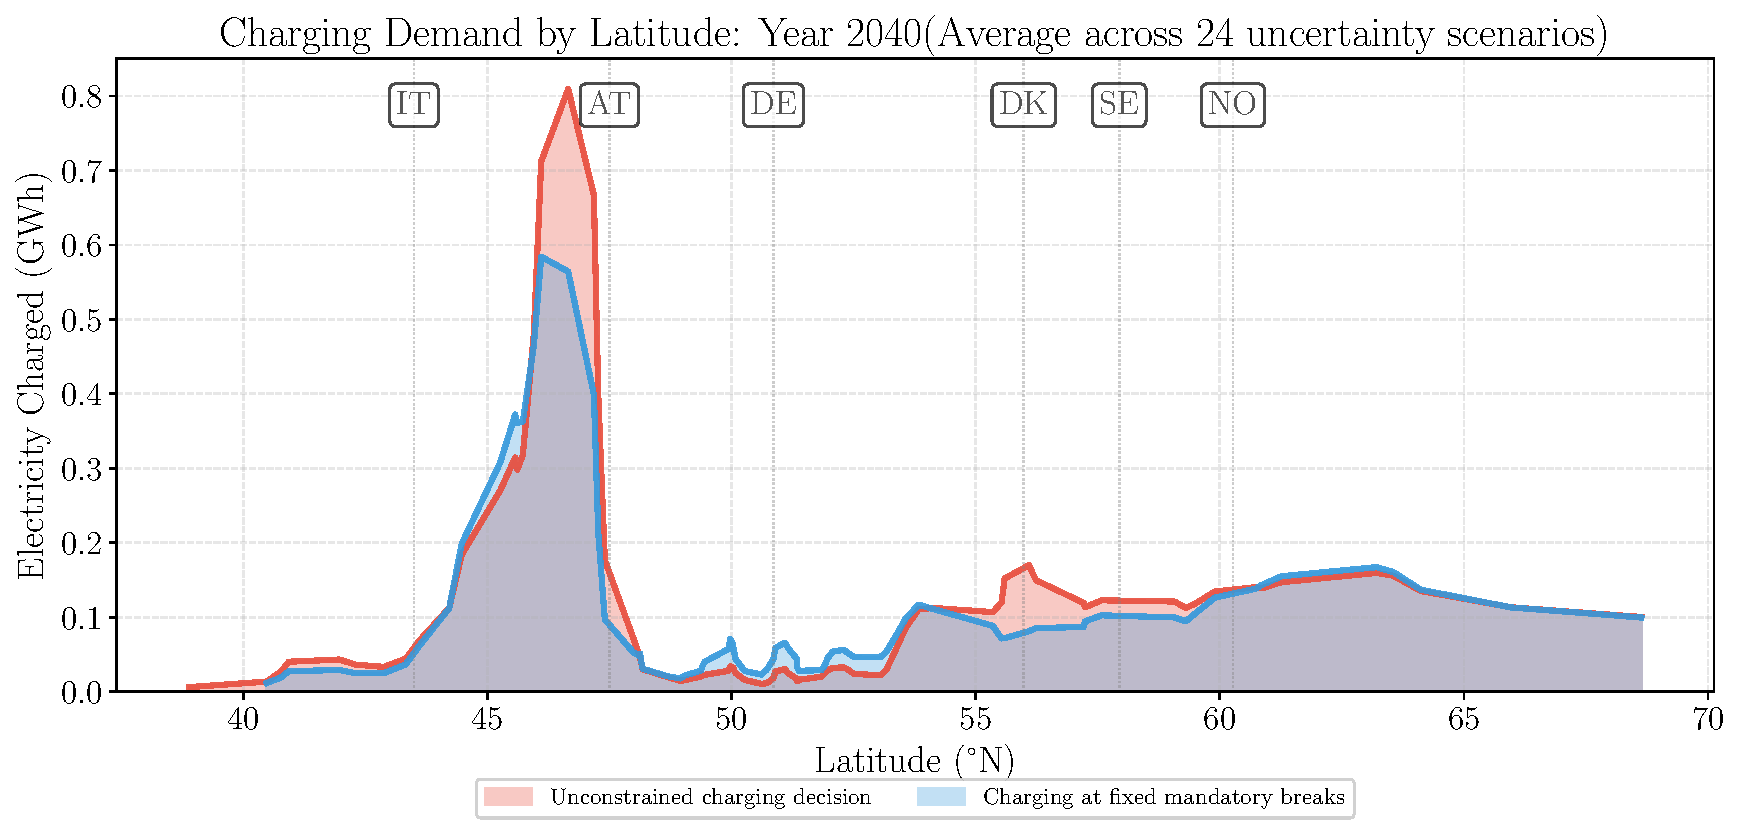
\includegraphics[width=0.8\linewidth]{images/charging_by_latitude_comparison_2040.pdf}
          \caption{Difference in charging demand allocation between the case in which the charging is not bound to fixed locations (\textit{Unconstrained charging decision}) and the case of being bound to fixed breaks positions (\textit{Charging at fixed mandatory breaks}) for the year 2040. The country codes indicate the average position of the centroid of the NUTS 2 regions by country along the Scandinavian-Mediterranean corridor.}
          \label{fig:distrib_charging_load}
    \end{figure}
    \hl{tell this story in words; increasing/decreasing charging loads; percentages in differences; to include this also in the conclusion; part of discussion: transferrability to other corridors: size and route and size of transport demand;}
    % Comparison: mandatory breaks only vs. flexible break-taking
    % How much spatial flexibility exists in charging load allocation?
    \begin{table}[H]
    \centering
    \caption{System cost comparison between scenarios.}
    \label{tab:cost_comparison}
    \begin{tabular}{@{}lr@{}}
    \toprule
    \textbf{Model run} & \textbf{System cost} \\ \midrule
    Unconstrained charging decision & 3647.58 \euro/1000tkm \\
    Charging at fixed mandatory breaks & 3647.80 \euro/1000tkm \\ \hline
    Absolute difference & 0.22 \euro/1000tkm\\
    Relative difference & 0.006\% \\ \bottomrule
    \end{tabular}
\end{table}


    \subsection{Levers to shift charging load spatially in the border region}
    % \hl{Here we look at one border regions that are particularly interesting}
   
    % We zoom in on the border region \textbf{DE-AT-IT}
    % and do some smaller analysis here: (1) The initial run (2) variable changes, (3) network changes; that is it - showing the results in a comparative bar plot 
    We now zoom in on the border region Germany-Austria-Italy, as we saw before, the BEV adoption there is particularly impacted by different electricity prices. This is also were a crucial part of the Scandinavian-Mediterranean corridor is allocated. Transportation routes between Germany and Italy go through a few transport connections through Austria, which are prone to congestion. We tested different settings to analyse which component of the charging cost could relocate or relieve the charging concentration along this bottleneck. In this analysis, the local costs were changed:
    \begin{itemize}
        \item \textit{Baseline} describes the GO RES electricity market price setting.
        \item In the \textit{Border Uniform Elec.} displays constant charging costs over this area.
        \item The \textit{Border Reversed Elec.} shows if the electricity prices in this area are allocated differently by country (only in the border regions), i.e., we resort here in such a way that the highest electricity price is assigned to lowest price and the regions of the lowest prices, the highest electricity price.
        \item In the \textit{Border Reversed Network}, constant network fees are assumed.
        \item The \textit{Border Reversed Network} follows the same analogy as the \textit{Border Reversed Elec.} scenario, but for network fees.
    \end{itemize}

    An important observation here is that particularly the variable price component (electricity price) are dominant in the concentration of the charging demand. The charging loads in Austria are succesfully decreased throughout all changes in charging cost components. 
    % \begin{itemize}
    %     \item clean bar plot just showing four snap shots 2028, 2036, 2040 ,2044 - showing all four 
    %     \item also: does this impact the adoption of BEVs? 
    % \end{itemize}
    \begin{figure}[H]
              \centering
              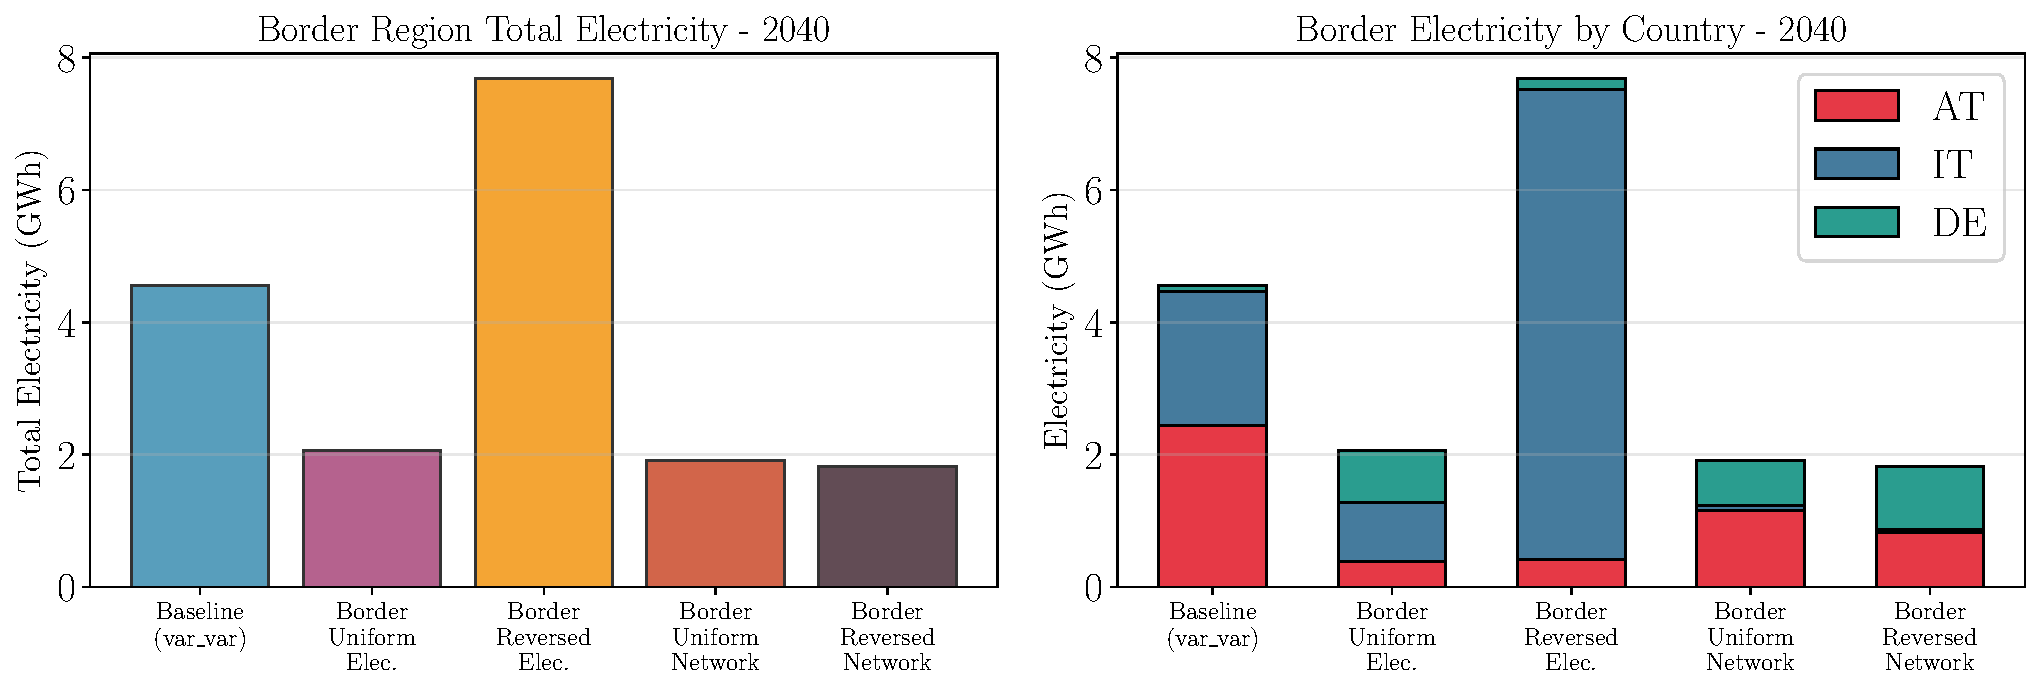
\includegraphics[width=1\linewidth]{images/border_sensitivity_scenario_000_2040.pdf}
              \caption{Change of charging demand distribution at Germany-Austria-Italy border through changed charging costs in border regions.}
              \label{fig:modalshift}
        \end{figure}
    % Testing different measures to influence spatial distribution of charging demand
    % Variable costs (electricity prices) vs. fixed costs (network fees) vs. other levers
    % \hl{Insert results on different levers to shift charging load: (1) electricity price variations, (2) network fees, (3) other policy measures. Which lever has the strongest effect on spatial redistribution?}

    \subsection{Modal shift to rail}
    % \begin{itemize}
    %     \item classic bar plot: mode shift + electrification 
    %     \item locations of mode shift 
    % \end{itemize}
    % % Impact of enabling modal shift towards rail on charging load distribution
    % % How does rail availability reduce/redistribute BEV charging demand?
    % \hl{Insert results on modal shift to rail: How does the availability of rail freight affect the spatial distribution of truck charging loads? To what extent can modal shift mitigate charging load concentration?}
    Figures \ref{fig:modalshift} and \ref{fig:modalshift_2} display results for modal shift. We here introduce that 30\% of the transport performance can be shifted to rail transport. Figure \ref{fig:modalshift_2} particularly shows how charging load is differently distributed along the corridor, indicating that cost-optimally transport volumes should be shifted to rail around Italy. 
    \begin{figure}[H]
              \centering
              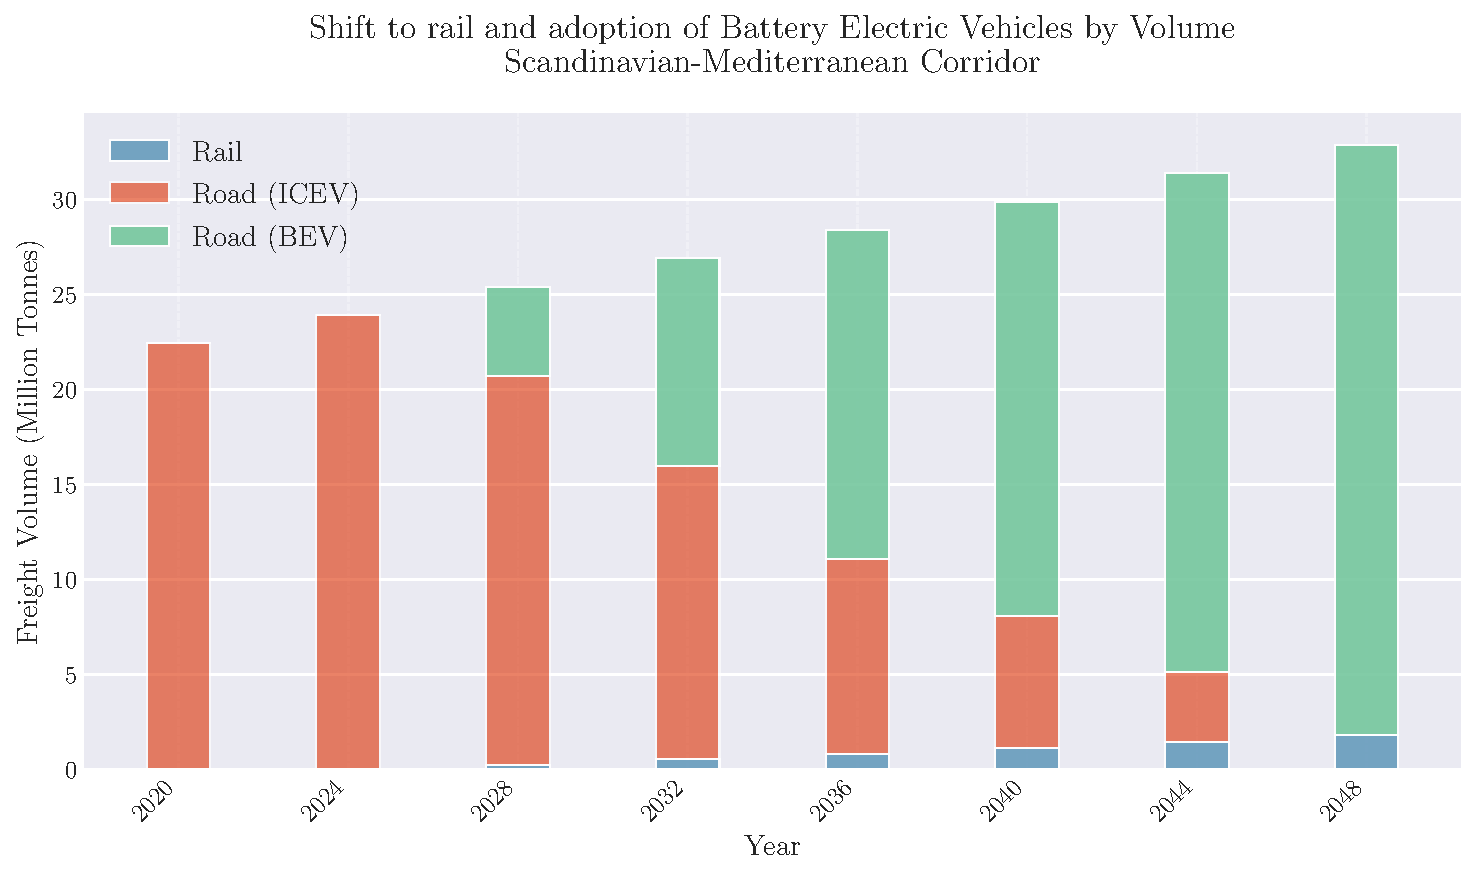
\includegraphics[width=0.8\linewidth]{images/modal_split_volume.pdf}
              \caption{\textit{Modal shift scenario:} Shift of road transport from trucks with internal combustion engine to rail mode and battery-electric trucks.}
              \label{fig:modalshift}
        \end{figure} 

    \begin{figure}[H]
              \centering
              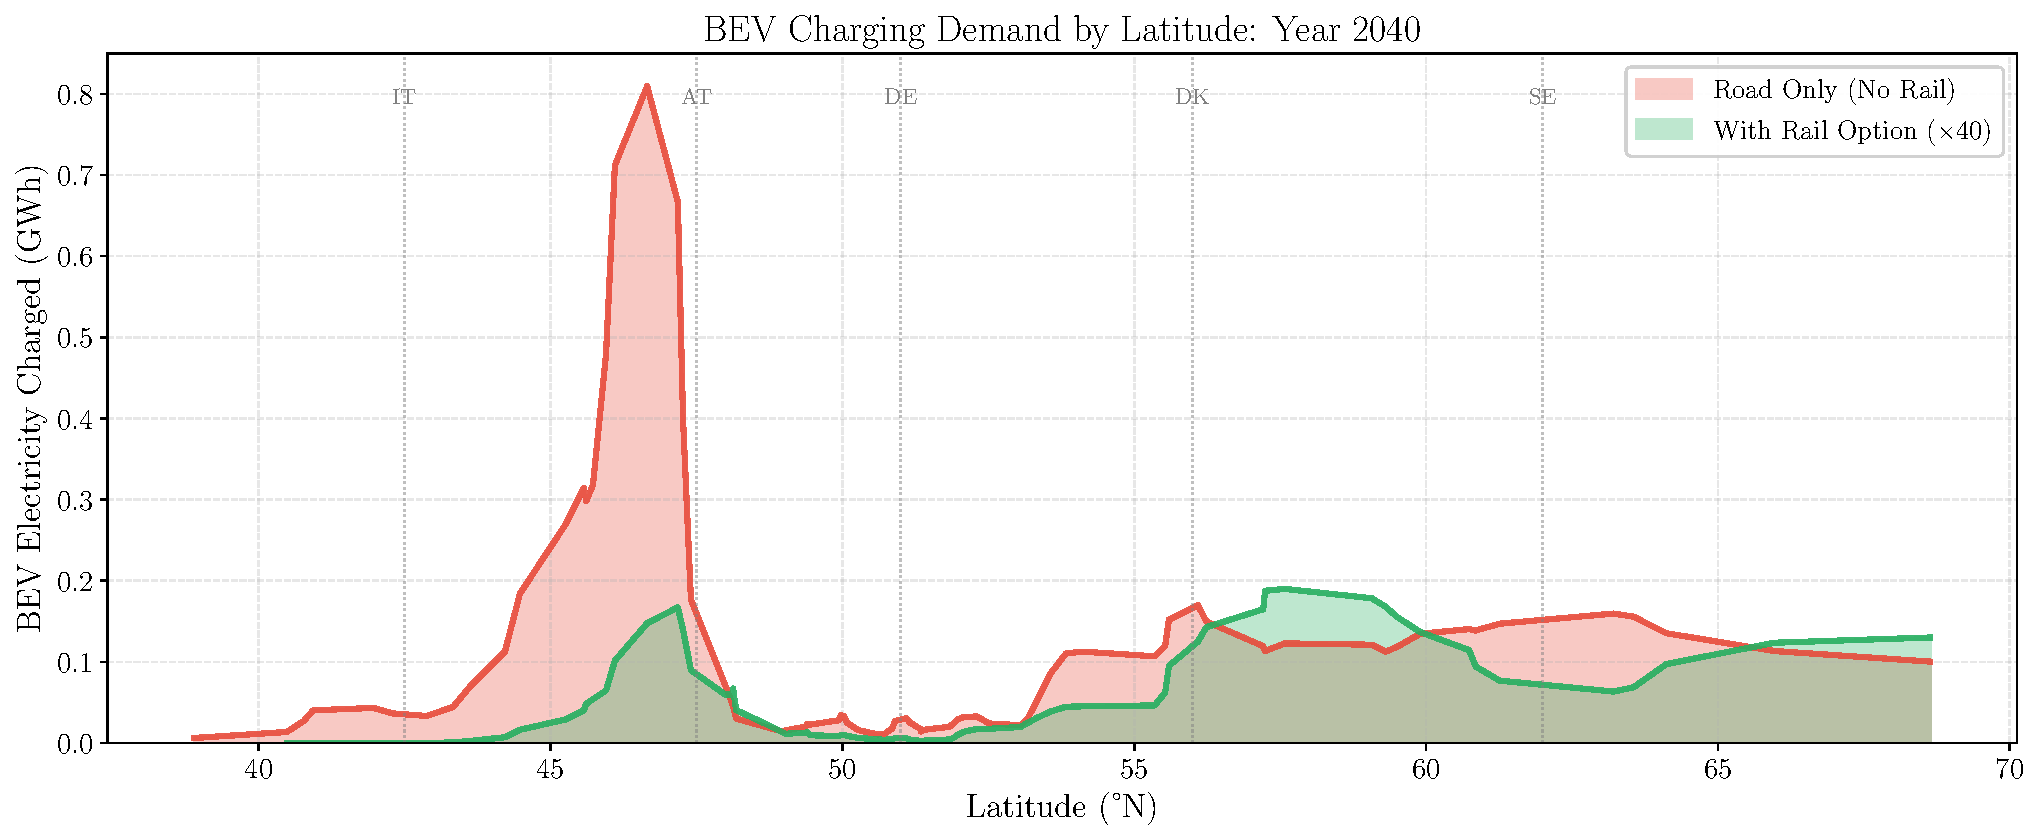
\includegraphics[width=0.8\linewidth]{images/bev_charging_by_latitude_rail_comparison.pdf}
              \caption{Comparison between baseline scenario and shift of charging demand of battery-electric trucks distribution by latitude through shift to rail mode.}
              \label{fig:modalshift_2}
        \end{figure}
    \hl{the costs are crucial, what is the incentive? Average may be also different for the ones that are changing; diving into the details; more detailed metrics: OPEX + the routes that are really impacted; OPEX or just charging costs }

    @time usage: include a constraint on this; maximum constraint on the travel time; giving some freedom; / include this maybe also as a results? Vot leveraged in the objective vs. hard constrain with 5\% allowance

    looking at valueing \hl{the spatial movements in the allocation}
% \section{Discussion}
    
%    \subsection{Impact of geographically varying charging costs}
%    \begin{itemize}
%        \item deviations from the initaial mandatory break locations
%        \item also leading to earlier adoption ( costs or technical performance?) 
%        \item the zoom-in has demonstrated how charging load can be effectively reallocated, based on the border region analysis; 
%        \item charging cost optimized charging behavior enables earlier adoption of battery electric trucks 
%        \item What are implications of this?
%        \begin{itemize}
%            \item for electricity system planning: 
%            \item for modeling of integration to electrificity system: flexibility provision cross-border flexibility
%            \item policy: network fees during the build-up direct the allocation of charging costs,  policy measures tackling the capacity installation costs are evidently effective to reallocate loads to other regions; also in the consideration of maybe dynamic pricing to exploit contribution towards balancing energy markets 
%        \end{itemize}
%        \paragraph*{Limitations} the linear modeling; no binaries; so half trucks and also not full break indicated with binaries; likely an overestimation of the flexibility demand 
%    \end{itemize}
%    \subsection{Mode shift to rail}
%    \dots how does the rail shift affect the allocation? shift is where its most expensive? so does it increase the concentration of demand? 
%    The shift to rail happens is allocated in regions with high charging costs. Therefore we see the the shhift to be primarily allocated in \dots s

%    \dots neglecting local restrcitions of deployment of rail infrastructure \dots avoiding 
\section{Discussion}
    \hl{\dots by research question}
\section{Conclusion}
    This work provides the first quantification regarding the role of interzonal differences of electricity prices and network fees on the charging demand allocation of battery-electric trucks in long-haul freight transport. While previous literature has addressed the spatial flexibility of charging demand allocation at smaller scopes, i.e., in the distribution grid or for singular transport routes, our analysis demonstrates that the cross-border consideration and allocation of demand beyond market zones is relevant between European market zones. 

    The results of this analysis has implications and future work on multiple levels.

    \paragraph{Electricity system planning}
    The shifting of loads across electricity market zones is an additional dimension (next to shifting in time) to be exploited in the design of policies supporting grid-friendly charging and the flexibility provision for balancing and congestion markets.
    
    \paragraph{Charging infrastructure planning}
        Supporting the electrification of the long-haul fleet needs to consider current international routes and allocate charging infrastructure capacities allowing for lower charging costs exploiting the flexibility along the route for. This should be considered in the large-scope planning of charging infrastructure for BETs in long-haul freight transport.
        %significantly faster adoption of Battery electric trucks by \hl{\dots} has been demonstrated. Moreover, 
    \paragraph{Future Work}
        Future work must include the three following analytical extensions:
        \begin{itemize}
            \item For the provision of flexibility, hourly differences in prices are the main price signal for demand-response. Beyond regionally differing absolute levels of electricity prices, the present modeling framework should be enhanced by representing intra-day volatility and the changes in it throughout the years through the expansion of renewable energy sources. This could enable us to study dynamic tariff structures and model the utilization of the charging infrastructure more realistically.

            \item Based on this, the modeling framework with the consideration of hourly or sub-hourly utilization of charging provision, together with the vehicle movements, must be considered together with an operational model of the electricity system to, on the one hand, quantify the impact of the geographically concentrated charging loads on the grid operation, and, on the other hand, analyse the potential of flexibility provision for balancing and congestion management.
            
            \item Concerning an alternative case study application, the geographic scope should be extended to multiple, if not all, transport corridors in the Trans-European Transport Network to study the large-scale potential and effects of charging-cost-optimal allocation of charging demand of European long-haul freight road transport. 

            \item The application to alternative market zone splitting should be performed to address the effect on the concentration of charging loads. A concrete example for this would be the highly-depated potential market zone splitting of Germany which would split the current Geman market zone into two vertically aligned market zones, in the North and the South. This would substantially impact the allocation of demand in the Scandinavean-Mediterranean corridor, as Germany is allocated centrally and most of the interantional freight along this corridor passes through the country.
        \end{itemize}
        


%% The Appendices part is started with the command \appendix;
%% appendix sections are then done as normal sections
\appendix
\bibliographystyle{plainnat} % or abbrvnat, unsrtnat
 \bibliography{interacttfqsample}
\subsection{Methodology and Data}

\subsubsection{Spatial aggregation of truck traffic}

The truck traffic for 2030 is given at high geographic resolution below NUTS-3 regions \cite{speth2021synthetic}. The data is aggregated to NUTS-2 level to improve the computation efficiency. This is done by accumulating origin-destination connections by origin and destination nodes which lie within the same NUTS-2 area. In this process, the tonnage is summed and distances along the route are averaged which is particularly relevant for the first and the last edge as the origin and destination nodes are not directly overlapping. The final transport demand in Tkm matches by 0.0\% of difference. The number of OD pairs was reduced from 603174 to 2928. Figure \ref{fig:aggregation} displays the change in distance distribution due to the aggregation. The average length of a route is 872.9 km at NUTS-3 resolution, and  1352.3 km at NUTS-3 resolution. The histogram indicates that through the aggregation, some significant long routes are excluded.

        \begin{figure}[H]
              \centering
              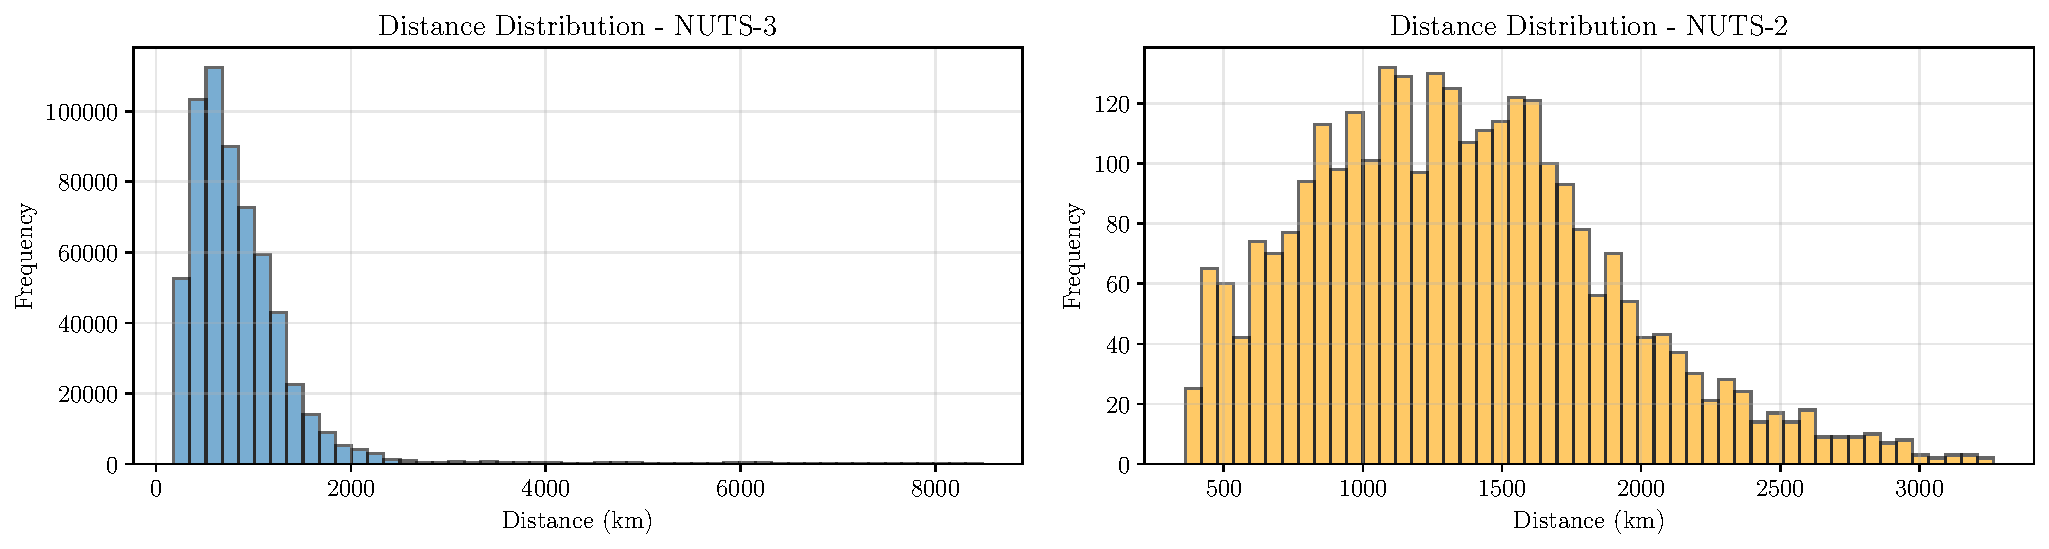
\includegraphics[width=1\linewidth]{images/aggregation_distance_distributions.pdf}
              \caption{Histogram of the distances of international routes in the case study area of the Scandinavian-Mediterranean transport corridor on two aggregation levels: NUTS-3 versus NUTS-2.}
              \label{fig:aggregation}
        \end{figure}
%  \hl{\textbf{TODO}: }
% \section{Example Appendix Section}
% \label{app1}

% Appendix text.

%% For citations use: 
%%       \citet{<label>} ==> Lamport (1994)
%%       \citep{<label>} ==> (Lamport, 1994)
%%

%% If you have bib database file and want bibtex to generate the
%% bibitems, please use
%%
%%  \bibliographystyle{elsarticle-harv} 
%%  \bibliography{<your bibdatabase>}

%% else use the following coding to input the bibitems directly in the
%% TeX file.

%% Refer following link for more details about bibliography and citations.
%% https://en.wikibooks.org/wiki/LaTeX/Bibliography_Management




%%
%% End of file `elsarticle-template-harv.tex'.


\end{document}